\documentclass[12pt]{report}

\usepackage[utf8]{inputenc}
\usepackage[T1]{fontenc}
\usepackage[french]{babel}
%Options: Sonny, Lenny, Glenn, Conny, Rejne, Bjarne, Bjornstrup
\usepackage[Conny]{fncychap}
\frenchbsetup{StandardLists=true}
\usepackage{graphicx}
\usepackage{enumitem}
\setlist[itemize]{label=\textbullet, topsep=0cm}
\setlist[description]{topsep=0cm}
% \setlist[description]{leftmargin=30pt,labelindent=\parindent}
\usepackage{mathpazo}
% \usepackage{fullpage}
\usepackage[a4paper, width=150mm, top=25mm, bottom=25mm]{geometry}
\usepackage[colorlinks=true, urlcolor=blue, linkcolor=blue]{hyperref}
\usepackage{parskip}
% \parskip=12pt 
% \parindent=0pt
\usepackage{fancyhdr}

\pagestyle{fancy}
\fancyhead{}
% \fancyhead[RO,LE]{Thesis Title}
% \fancyhead[L]{\rightmark}
\fancyhead[C]{\leftmark}
\fancyfoot{}
\fancyfoot[C]{\thepage}
% \fancyfoot[LO,CE]{Chapitre \thechapter}
% we can use \leftmark and \rightmark to add chapter title and section title to header or footer with \fancyhead or \fancyfoot.
% \fancyfoot[CO,RE]{Author Name}
\renewcommand{\headrulewidth}{0.4pt}
% \renewcommand{\footrulewidth}{0.4pt}

\usepackage[defaultlines=4,all]{nowidow}
\usepackage{caption}
\usepackage{subcaption}
\usepackage{verbatim}
\usepackage{booktabs}
\usepackage{listings}
\lstset{
  columns=fullflexible,
}
\usepackage{soul}
\usepackage{shadow}
\usepackage{float}
% \title{
%     {Thesis Title}\\
%     {\large Institution Name}\\
%     {
\includegraphics[scale=1]{images/USTHB_Logo.png}}
% }
% \author{Malaoui Sidahmed \and Salim Bitam}
% \date{\today}

\begin{document}

%!TEX root = ../main.tex

\begin{center}
    \normalsize{Ministère de l'Enseignement Supérieur et de la Recherche Scientifique}\\
    \normalsize{Université des Sciences et de la Technologie Houari Boumediene}\\
    \normalsize{Faculté d'électronique et d'informatique}\\
    \normalsize{Département d'informatique}\\
    \end{center}
    \begin{center}
    
\includegraphics[width=4cm,height=4cm]{images/USTHB_Logo.png}
    \end{center}


    \begin{center}
    \Huge{\textbf{Mémoire de Licence}}\\
    \large{Domaine Informatique}\\
    \textbf{}\\
    \large{\textbf{Option: Informatique}}\\
    \textbf{}\\
    \bigskip
    \normalsize{\textbf{Thème}}
    \end{center}
    \shabox{
    \begin{minipage}{0.9\textwidth}
    \begin{center}
    \Large{Étude et développement de malware}
    \end{center}
\end{minipage}
}
\\
\\
\\
\begin{table}[h]
    \center
    \begin{tabular}{p{8cm}p{6.5cm}}
    \textbf{Présenté par :} & \textbf{Sujet proposé par :}\\
    - \textsc{Bitam} Salim  & - \textsc{Zeraoulia} Khaled \\
    - \textsc{Malaoui} Sidahmed Bilal  & \\
    \end{tabular}
\end{table}
\\
\\

\begin{table}[h]
    \begin{tabular}{p{6.5cm}p{5cm}}
    \textbf{Devant le jury composé de:}&\\
    - \,\,\, Mr. \textsc{Belkhir} & Président \\
    - \,\,\, Mme. \textsc{Chenait} & Membre \\
    \end{tabular}
\end{table}

\vspace{2cm}
\begin{center}
Projet N : 217/2016
\end{center}

\clearpage

\pagenumbering{roman} 

\section*{Résumé} 
L’information est aujourd’hui devenue la plus grande richesse que toute personne ou entreprise peut posséder, et la sensibilité de ces mêmes informations a fait de la sécurité informatique une priorité majeure des individus et des professionnels.

Mais la naïveté de l’être humain l’a poussé à penser que sécuriser sa machine est amplement suffisant pour être à l’abri des attaques, il oublie cependant que sa machine est très souvent en interaction avec d’autres machines de sécurité moindre.

Dans cette étude, nous tenterons de mieux comprendre le fonctionnement des Virus, leurs méthodes d'infection et de propagation. Au vu de développer un Malware combinant un virus et une porte dérobée puis de tester sa propagation d'une machine de faible sécurité vers une machine sécurisée, et de tester son efficacité contre cette dernière. %vérifié

\section*{Abstract}
The information has now become the greatest asset that any person or company can own , and the sensitivity of this information has made computer security a major priority for individuals and professionals.

But the naivety of the human being led him to think that securing his own machine is  enough to be safe from attack , however, he forgets that his machine is very often in interaction with other lesser security machines.

In this study, we will try to better understand how the virus works , and their methods to infect and to propagate. In order to develop a Malware, combining a Virus and a Backdoor then test its spread from a low security machine to a secured machine and test its effectiveness against the latter. %vérifié

\paragraph{Mots clés :} Malware, Virus, Backdoor, Infection virale, Propagation.


\chapter*{Dédicaces}
Je dédie ce travail à mes parents qui m'ont toujours supporté et qui ont toujours sacrifié pour moi. Tout ce que
je pourrai faire pour eux n'atteindre même pas le quart de ce qu'ils m'ont donné et de ce qu'ils m'ont fait.

À ma chère famille, surtout mon petit frère et ma sœur.

À mes chers amis, Nassraddine, Lamine, Idris, Rabah, Habib, Walid, Hawas.

J'aimerai aussi et surtout dédié ce modeste travail à mes chers frères et sœurs Palestiniens qui sont opprimés par les
sionistes, les sionistes qui n'ont pas la moindre particule de noblesse ou de courage. Je dis au peuple Palestinien
que ça me fait mal au cœur de vous voir souffrir et de ne rien pouvoir faire, et ça me fait encore plus mal que 
les gouvernements qui prétendent être musulmane vous faite du mal et conspirent contre vous au-lieu de vous aider, tous 
ça pour gagner la bénédiction de leurs maîtres. 
Mais bi idni Allah, nous continuerons de nous développer pour pouvoir vous être utile dans un future proche.

Je dédie aussi ce travail aux peuples opprimés à travers le monde entier, peu importe leurs religions, peu importe
leurs origines. L'injustice reste de l'injustice, peu importe qui est l'oppresseur, peu importe qui est l'oppressé.

\vfill
Sidahmed
\vfill
\newpage
Je dédie ce travail à mes très cher parents qui m'ont toujours supporté dans mes moment difficile et qui se sont toujours sacrifié pour moi, à mon merveilleux père qui ma offert aide, patience et conseils, et ma merveilleuse mère dont les mots ne peuvent décrire, qui ma apporter un soutien morale et des conseils inestimable.

À ma chère famille, dont mes sœurs  adorées

À mes chers amis, Zaki, Ahmed, Sidahmed.

J'aimerai aussi et surtout dédié ce modeste travail à mes chers frères et sœurs Palestiniens qui sont opprimés par les
sionistes, les sionistes qui n'ont pas la moindre particule de noblesse ou de courage. Je dis au peuple Palestinien
que ça me fait mal au cœur de vous voir souffrir et de ne rien pouvoir faire, et ça me fait encore plus mal que 
les gouvernements qui prétendent être musulmane vous faite du mal et conspirent contre vous au-lieu de vous aider, tous 
ça pour gagner la bénédiction de leurs maîtres. 
Mais bi idni Allah, nous continuerons de nous développer pour pouvoir vous être utile dans un future proche.

Je dédie aussi ce travail aux peuples opprimés à travers le monde entier, peu importe leurs religions, peu importe
leurs origines. L'injustice reste de l'injustice, peu importe qui est l'oppresseur, peu importe qui est l'oppressé.
\vfill
Salim
\vfill

\chapter*{Remerciements}
Nous voudrons commencer par remercier \textsc{dieu}, le miséricordieux, qui nous a donnée les moyens et la force
d'aller jusqu'au bout de ce projet.

Nous sommes très reconnaissants à Monsieur \textsc{Belkhir} et Madame \textsc{Chenait} d'avoir accepté de juger notre travail.

Nous tenons à remercier notre promoteur Monsieur \textsc{Zeraoulia} Khaled pour son soutient.

Un très grand merci à Monsieur \textsc{Adda} Mohamed pour son soutient et son aide précieux.

Nous voudrons aussi remercier le département de l'informatique d'ELIT, de nous avoir accordé un moment précieux de
leurs temps inestimable.

Enfin, nous remercions tous ceux qui ont contribué de près ou de loin à la réalisation de ce projet.


\renewcommand{\contentsname}{Sommaire}
\tableofcontents
\listoffigures
\listoftables

\chapter*{Introduction Générale}
\pagenumbering{arabic} %Pour réutiliser la numérotation des pages.
\addcontentsline{toc}{chapter}{\protect\numberline{}Introduction générale}


%Here is how to add figures. ===========================================================================================
% \begin{figure}[h]
%     \centering
%     \includegraphics[scale=1]{images/msf_example.jpg}
%     \caption{Figure example}
%     \label{Figure example}
% \end{figure}

%Here is how to add subfigures. ========================================================================================
% \begin{figure}
%     \centering
%     \begin{subfigure}[b]{0.3\textwidth}
%         \centering
%         \includegraphics[width=\textwidth]{images/example01}
%         \caption{$y=x$}
%         \label{fig:y equals x}
%     \end{subfigure}
%     \hfill
%     \begin{subfigure}[b]{0.3\textwidth}
%         \centering
%         \includegraphics[width=\textwidth]{images/example02}
%         \caption{$y=3sinx$}
%         \label{fig:three sin x}
%     \end{subfigure}
%     \hfill
%     \begin{subfigure}[b]{0.3\textwidth}
%         \centering
%         \includegraphics[width=\textwidth]{images/example03}
%         \caption{$y=5/x$}
%         \label{fig:five over x}
%     \end{subfigure}
%     \caption{Three simple graphs}
%     \label{fig:three graphs}
% \end{figure}

% Document begin =======================================================================================================
\chapter{Introduction à la sécurité informatique et aux Malwares}
%!TEX root = ../main.tex

% Changer l'introduction (car vous avez ajouter le hacking)
Le premier chapitre de ce mémoire portera sur quelques notions et concepts de base de la 
sécurité informatique, à l’effet d’éclaircir et de définir une terminologie et un vocabulaire 
spécifique à ce domaine d’activité. %vérifié

\newpage

\section{Généralités sur la sécurité des systèmes informatiques}
    \subsection{Introduction}
    Dans les temps anciens, les besoins des gens étaient simples : nourriture, eau, abri, et la chance occasionnelle
    de propager l'espèce. Leurs besoins de base n'ont pas changé, mais les façons dont elles sont comblées ont changé.
    La nourriture est achetée dans des magasins qui sont alimentés par des chaînes d'approvisionnement avec des
    systèmes d'inventaire informatisés ; l'eau est distribuée à travers des systèmes contrôlés par des ordinateurs ; 
    les abris sont achetés et vendus par des agents immobiliers maniant des ordinateurs.
    La production et la transmission d'énergie pour faire fonctionner tous ces systèmes est contrôlé par des
    ordinateurs, et c'est les ordinateurs qui sont utilisés pour gérer les transactions financières pour le 
    payement de tout cela. \cite{virus} %vérifier

    Ce n'est pas un secret que l'infrastructure de la société repose sur des ordinateurs maintenant.
    Malheureusement, cela signifie qu'une menace envers les ordinateurs est une menace envers la société. 
    Mais quels sont les problèmes auxquels les infrastructures essentielles et critiques sont-elles confrontées.%vérifié

    \subsection{Types de menaces}
    Il y a quatre principales menaces à considérer. Ce sont les quatre cavaliers de l'apocalypse électronique :%vérifié
    \begin{description}
        \item[Spam :] Le terme couramment utilisé pour décrire les courriers électroniques non sollicités envoyés 
            en grand nombre à des boîtes aux lettres électroniques ou à des forums, dans un but publicitaire 
            ou commercial. Les statistiques varient au fil du temps, mais suggèrent que plus de 
            70\% du trafic des courriers électroniques tombe dans cette catégorie.%vérifié
        \item[Bugs :] Ce sont des erreurs logicielles qui, quand elles surgissent, peuvent faire crasher votre 
            logiciel immédiatement, si vous êtes chanceux. Elles peuvent également entraîner une corruption de données,
            des failles de sécurité, et des problèmes très difficiles à trouver. \cite{virus} %vérifié
        \item[Dénis de service (DoS):] Ce type de menace affame l'utilisation légitime des ressources ou des 
            services. Par exemple, une attaque DoS peut utiliser tout l'espace disque disponible sur un 
            système, de sorte que les autres utilisateurs ne pourront pas faire usage de celui-ci ; comme elles
            peut générer des ramettes de trafic réseau afin que le trafic légitime ne puisse pas passer à travers.
            Les attaques DoS simples sont relativement faciles à mettre en place, il suffit tout simplement 
            de submerger une machine avec des requêtes qui ont l'air d'être légitimes. \cite{virus} %vérifié
        \item[Logiciels malveillants (Malware) :] Ce sont des logiciels dont l'intention est malveillante, 
            ou dont l'effet est malveillant. Le spectre des logiciels malveillants couvre une grande variété 
            de menaces spécifiques, y compris les virus, les vers, les chevaux de Troie et les logiciels espions.
            \cite{virus}%vérifié
    \end{description}

    L'étude dans cette thèse sera portée sur les Malwares et les techniques employés par ces derniers pour propager
    et cacher leurs présences dans un système. %vérifié

    \subsection{L'illusion de la sécurité absolue}
    Évidemment, tout le monde veut que leurs ordinateurs soient sécurisés contre les menaces. Malheureusement, 
    la sécurité absolue n'existe pas. Vous pouvez prendre beaucoup de précautions techniques pour protéger vos 
    ordinateurs, mais vos protections sont peu susceptibles d'être efficaces contre un attaquant déterminé avec
    assez de ressources. Comme exemple, un attaquant déterminé pourrait conduire un camion à travers le 
    mur de votre bâtiment et voler vos ordinateurs. 
    Pour faire simple, aucun système n'est infaillible, et aucune information n'est à l'abri, c'est juste une
    question de volonté et de ressources. \cite{virus} %vérifié

    Même si aucun système ne peut être sécurisé d'une manière absolue, une sécurité relative peut être considérée
    en fonction de six facteurs : %vérifié
    \begin{itemize}%[label=$\star$]
        \item Quelle est l'importance de l'information qui est protégée ?
        \item Quel est l'impact potentiel, si la sécurité est violée ?
        \item Qui voudra obtenir cette information ?
        \item Quelles sont les compétences et les ressources disponibles à l'attaquant ?
        \item Quelles sont les contraintes imposées par l'usage légitime ?
        \item Quelles sont les ressources disponibles pour mettre en œuvre la sécurité ?
    \end{itemize} %vérifié

    Diviser le concept de la sécurité de cette manière modifie le problème. La sécurité n'est plus une question 
    binaire dont les deux choix possibles sont : sécurisé ou non-sécurisé, mais plutôt une gestion des risques.
    L'implémentation de la sécurité peut être considérée comme le compromis entre le niveau de protection, 
    la facilité d'utilisation du système, et le coût de l'implémentation. \cite{virus} %vérifié

    \subsection{Les objectifs de la sécurité informatique}
    La sécurité informatique consiste en générale à assurer que les ressources matérielles ou logicielles sont 
    uniquement utilisées dans le cadre prévu. La sécurité informatique vise généralement cinq principaux objectifs :
    %vérifié
    \begin{description}
        \item[L'intégrité :] Consiste à déterminer si les données n'ont pas été altérées durant la communication 
            (de manière fortuite ou intentionnelle).
        \item[La confidentialité :] Consiste à rendre l'information inaccessible à d'autres personnes que les 
            seuls acteurs de transaction.
        \item[La disponibilité :] L'objectif de la disponibilité est de garantir l'accès à un service 
            ou à des ressources.
        \item[La non-répudation :] La non-répudation de l'information est la garantie qu'aucun des correspondants 
            ne pourra nier la transaction.
        \item[L'authentification :] Consiste à assurer l'identité d'un utilisateur, et bien garantir que chaque
            personne est celui qu'il prétend être.
    \end{description} %vérifié

    \subsection{Les attaques informatiques}
    Une attaque informatique est une attaque offensive pour l’exploitation des systèmes informatiques, 
    des entreprises, et des réseaux, est-ce par divers moyens d’actes malveillants. 
    Il existe de multiples catégories d’attaques informatiques dont les buts et les techniques différents. %vérifié
    \begin{description}
        % \item[Interruption :] Avec ce type d'attaque, un atout du système est détruit ou mis hors d'état d'utilisation.
            % C'est une attaque portée à la \emph{disponibilité}. Exemples : la destruction d'une pièce matérielle, 
            % la coupure d'une ligne de communication, ou la mise hors service d'un système de gestion de fichiers.
        \item[Interruption :] Ce type d'attaque vise la \emph{disponibilité}. Il s’agit de compromettre les 
            ressources physiques ou logiques d'un système. Exemple : les attaques \emph{DoS} et \emph{mac flooding}.
            %vérifié
        \item[Fabrication :] Ce type d’attaque vise l'\emph{authenticité}. Il s'agit de l’ajout d’une 
            information contrefait au système. Exemple : l'attaque \emph{ARP cache poisoning}. %vérifié
        \item[Interception :] Ce type d’attaque vise la \emph{confidentialité}. Il s’agit de l'acquisition de données 
            destinées a autrui. Exemple : l’attaque \emph{sniffing}. %vérifié
        \item[Modification :] Ce type d’attaque vise l'\emph{intégrité}. Il s’agit de la modification 
            de données d’un programme pour changer/altérer le fonctionnement ou le comportement de ce dernier. 
            Exemple : attaque par injection de code. %vérifié
    \end{description}
    
\section{Le Hacking}
    Le hacking \cite{bases_hacking} est l'art et la manière de modifier un élément physique ou virtuel 
    de sorte à ce que celui-ci n'ait pas le comportement prévu initialement par ses créateurs. %vérifié

    Démarrer une voiture sans clé est du hacking de la même façon que cracker le mot de passe de la session 
    d'un utilisateur ou accéder à des informations cryptées. Tout ce qui n'était pas prévu par le concepteur et 
    qui a été détourné de toute forme qui soit est du hacking. %vérifié

    Le hacking ne se résume donc pas au cracking wifi du voisin ou à la prise de possession de l'ordinateur 
    d'une victime. %vérifié

    Les hackers sont des personnes bien ou mal intentionnées qui utilisent leurs connaissances pour exploiter 
    des failles dans des environnements distincts afin d'effectuer des modifications entraînant une attitude 
    différente de celle que l'auteur a prévu pour pouvoir en tirer un avantage. %vérifié

    Cela peut paraître néfaste ; et ça l'est dans certains cas. Cependant, sans les hackers, internet ne prendrait 
    pas la tournure qu'il est en train de prendre, à savoir une tournure open source et communautaire, 
    déliée des pouvoirs qui tentent de se l'accaparer. \cite{hacking} %vérifié

    \subsection{Différents type de hacker}
    Il existe différents types de hackers dans le monde de la sécurité informatique. On y trouve : %vérifié
    \cite{types_de_hacker}

    \begin{description}
        \item[Les gamins des scripts :] Aussi appelé \emph{Script Kiddie}. 
            Ce sont des personnes qui utilisent des outils, des scripts, et des programmes
            créés par des vrais hackers. Dans des mots plus simples, ce sont ceux qui ne savent pas comment 
            les systèmes marchent, mais qui arrivent quand même à les exploiter en utilisant des outils qui 
            existent déjà. %vérifié

        \item[Les hackers aux Chapeaux Blancs :] Aussi appelé \emph{White Hat Hackers}.
            Ce sont les gars gentils qui utilisent le hacking pour défendre. 
            Le but principal d'un hacker au chapeau blanc est d'améliorer la sécurité des systèmes, en trouvant
            des failles de sécurités et les fixer. Ils travaillent pour des organisations ou individuellement, pour 
            rendre le cyberespace plus sécurisé. 

            Le slogan de cette catégorie de hacker est : \emph{Apprendre l'attaque pour mieux se défendre}. %vérifié
            
        \item[Les hackers aux chapeaux noirs :] Aussi appelé \emph{Black Hat Hackers}.
            Ce sont vraiment les mauvais gars, qui ont des intentions malicieuses. Ils utilisent le hacking 
            pour voler de l'argent, infecté des systèmes avec les Malwares (\autoref{malwares}) \ldots{} etc. %vérifié

        \item[Les hackers aux chapeaux gris :] aussi appelé \emph{Grey Hat Hackers}.
            Ce sont des hackers qui n'ont pas d'intentions malicieuses, mais qui tentent quand même de pénétrer 
            un système dont ils n'ont pas l'autorisation d'accès, juste pour le plaisir ou pour démontrer 
            l'existence d'une faille de sécurité. %vérifié

        \item[Les Hacktivists :] Les hackers appartenant à cette catégorie, utilisent leurs compétences pour 
            dénoncer l'injustice et/ou attaquer le système ou le site web d'une entité responsable d'une injustice. 
            L'un des Hacktivists le plus connu est \emph{Anonymous}. %vérifié
    \end{description}

    \subsection{Les phases d'un hacking réussi}
    Il y a en tout cinq grandes phases, qui lorsqu'elles sont accomplies avec succès, garantissent presque 
    toujours un hacking \cite{bases_hacking} réussi. Le hacker devra donc les couvrir une 
    par une et en tirer des conclusions. %vérifié

    Les cinq phases du hacking sont les suivantes \cite{phases_of_hacking} : %vérifié
    \begin{description}
        \item[La reconnaissance :] C'est la phase primaire où le hacker essaye de collecter autant d'informations que
        possible sur la cible. Ça inclut l'identification de la cible, trouver les adresses IP \cite{reseau}
        de la cible \ldots{} etc. %vérifié

        \item[Le scan :] Ça consiste à prendre les informations découvertes durant la phase de reconnaissance, et 
            les utilisés pour examiner le réseau de la cible. Les outils qui peuvent être utilisés par 
            le hacker durant cette phase sont les scanners de ports et les scanners de vulnérabilités. %vérifié

        \item[Le gain d'accès :] Après le scan, le hacker modélise le plan du réseau de la cible avec l'aide
            des données récoltées pendant les deux phases précédentes. C'est la 
            phase où le vrai hacking se déroule. Les vulnérabilités découvertes durant les phases précédentes sont 
            maintenant exploitées pour gagner un accès à la cible. %vérifié

        \item[Le maintien d'accès :] Une fois le hacker a gagné l'accès à la cible, la prochaine étape consiste à 
            maintenir cet accès pour une future utilisation. %vérifié

        \item[La couverture des traces :] Une fois le hacker a pu gagner et maintenir l'accès, il couvre ses traces 
            pour éviter qu'il soit détecter par les personnels de la sécurité, pour continuer d'utiliser le système.
            Les hackers essayent de supprimer toute trace de l'attaque, comme les fichiers journaux ou 
            les alarmes des systèmes de détections d'intrusions. %vérifié

    \end{description}

    \subsection{Les vulnérabilités}
    Les vulnérabilités sont des points faibles par lesquels l'intégrité d'un système peut être atteinte. Ces points 
    faibles ne sont pas toujours exploitables ; cependant, elles peuvent être combinées pour 
    réussir une exploitation. %vérifié
    
    Les vulnérabilités peuvent être exploitées pour infiltrer un système, ou pour obtenir des privilèges supplémentaires
    sur des systèmes déjà atteints. Elles peuvent être exploitées automatiquement par les Malwares 
    (\autoref{malwares}), ou manuellement par des personnes visant directement un système. %vérifié

    Les vulnérabilités se divisent en deux catégories, selon l'endroit où elles se situent : %vérifié
    
    \begin{description}
        \item[Vulnérabilités techniques :] Elles proviennent souvent de la négligence ou de l'inexpérience d'un 
            programmeur. Une vulnérabilité de cette catégorie permet généralement à un attaquant de duper 
            une application, par exemple en outrepassant les vérifications de contrôle d'accès ou en exécutant
            des commandes sur le système hébergeant l'application.
            \label{buffer_overflow} %vérifié

            Quelques vulnérabilités techniques surviennent lorsque l'entrée d'un utilisateur n'est pas contrôlée,
            permettant l'exécution de commandes ou de requêtes. D'autres proviennent d'erreurs d'un programme
            lors de la vérification des tampons de données (qui peuvent être dépassés), 
            causant ainsi une corruption de la pile mémoire
            (et ainsi permettre l'exécution de code fourni par l'attaquant). \cite{vulnerabilites} %vérifié

        \item[Vulnérabilités humaines :] Les humains sont le maillon le plus faible dans la chaîne de sécurité.
            Les humains peuvent oublier d'appliquer des patchs de sécurité critique, introduire des bugs
            exploitable, configurer mal leurs logiciels au point de les rendre vulnérables \ldots{}
            Il existe même une catégorie d'attaque dédiée à duper les individus, appelée \emph{ingénierie sociale} 
            \cite{bases_hacking}. %vérifié
    \end{description}

\section{Les Malwares} \label{malwares}
    Le mot \emph{Malware} est une abréviation de \emph{\textbf{mal}icious soft\textbf{ware}}, qui signifie 
    \emph{logiciel malveillant}. Un Malware est un logiciel qui peut être utilisé pour compromettre le
    fonctionnement des ordinateurs, voler des informations ou des données, contourner les contrôles d'accès
    \ldots{} etc. Dans la partie qui suit, les types les plus courants des Malwares seront abordés avec une explication 
    de leurs modes de fonctionnement et de leurs objectifs principaux. \cite{malware_types}%vérifié

    \subsection{Les types des Malwares}
    \begin{description}
        \item[Bombe logique :] Une bombe logique est un code constitué principalement de deux parties :
            \begin{enumerate}
                \item Une \emph{charge utile}, qui est l'action à effectuer. La charge utile peut être n'importe quoi,
                    mais puisque c'est un logiciel malveillant, la charge a généralement un effet malicieux.
                \item Une \emph{gâchette}, qui est une condition booléenne qui indique le moment du lancement de la
                    charge. La vraie limite de la charge est limitée seulement par l'imagination, et peut être basé sur
                    des conditions comme la date, le nom de l'utilisateur connecté, la version du système d'exploitation
                    \ldots etc.
            \end{enumerate}
            Une bombe logique peut être insérée dans un code existant, comme elle peut être autonome. 
            Ci-dessous un pseudo code exemple d'une bombe logique insérer dans un code existant :
            \begin{verbatim}
                instructions
                if condition is True:
                    executer_charge()
                instructions
            \end{verbatim}
            Une bombe logique peut être discrète et très difficile à trouver, surtout si elle s'y trouve parmi des 
            millions de lignes de code, et elle peut être utilisée facilement pour causer des 
            dégâts phénoménaux. \cite{virus} %vérifié

        \item[Virus :] Un virus informatique est un programme parasite généralement de petite taille, 
            doté d’une capacité d’infection et de multiplication, et possède une fonction nocive appelée 
            \emph{Payload}\footnote{Le terme Payload (charge utile en français) au figuré pour désigner 
            la partie du code exécutable d'un virus qui est spécifiquement destinée à nuire.}.

            La fonction d'infection permet au virus de s'introduire dans des fichiers de programme, 
            dans des fichiers de données utilisant un langage de script ou dans le secteur de démarrage 
            d’un disque dur. Lors de l'accès à ces programmes ou secteur, le code du virus s'exécutera de 
            façon d'abord silencieuse (phase de multiplication pendant laquelle il infectera d'autres fichiers) 
            puis visible (activation de la fonction nocive). %vérifié

            La fonction nocive pourra être déclenchée par un événement particulier, elle peut se limiter 
            à l'affichage d'un message agaçant ou, plus généralement, conduire à des perturbations graves 
            de l'ordinateur comme des ralentissements du fonctionnement, effacement ou corruption de 
            fichiers ou pire encore le formatage du disque dur. \cite{virus_informatique} %vérifié
% J'ai ajouté cette partie.

            Ci-dessous se trouve un pseudo code exemple d'un virus informatique :
            \begin{verbatim}
                def virus():
                infecter()
                if gachette() is True:
                    executer_charge()
            \end{verbatim}

        \item[Ver :] Un ver informatique est un programme autonome qui peut s'auto-reproduire, 
            et qui ne repose pas sur d’autre exécutable. Il se propagent d'une machine à travers les 
            réseaux en profitant des ports ouverts, mais la méthode la plus classique consiste à s'introduire 
            sous la forme d'une pièce jointe attachée à un mail.

            Un ver ne se multiplie pas localement, contrairement aux virus, mais sa méthode la plus 
            habituelle de propagation consiste à s'envoyer dans des mails générés automatiquement. 
            Ces mails sont expédiés à l'insu de l'utilisateur vers diverses adresses. 
            Ces adresses sont généralement prélevées par le ver dans les fichiers présents sur le disque

            Les vers installent généralement sur l'ordinateur d'autres programmes nocifs : comme les logiciels 
            espions, les Keyloggers, et les portes dérobées. \cite{ver_informatique}

        \item[Porte dérobée :] \label{backdoor} Une porte dérobée est n'importe quel mécanisme qui peut contourner un
            contrôle de sécurité ordinaire. Les programmeurs créent dés fois des portes dérobées pour 
            des raisons légitimes, telles que passer une procédure d'authentification coûteuse lors 
            de débogage d'un service réseau.

            Comme les bombes logiques, les portes dérobées peuvent être insérées dans un code existant, comme elle
            peuvent être autonomes. Ci-dessous se trouve un pseudo code exemple d'une porte dérobée insérer dans 
            un code existant :
            \begin{verbatim}
                nom_utilisateur = lecture()
                mot_de_pass = lecture()
                if nom_utilisateur = "créateur de la porte dérobée":
                    laissee_entree()
                if est_valide(nom_utilisateur) and 
                        est_valide(mot_de_pass):
                    laissee_entree()
                else:
                    renvoyer()
            \end{verbatim}

            Il existe un type spécial des portes dérobées, appelé \emph{RAT}\footnote{Le mot RAT est une
            abréviation de \emph{Remote Access Tool} qui signifie outil d'accès à distance.}. Ce type de portes
            dérobées donne un accès total à un ordinateur pour un contrôle à distance. L'utilisateur peut
            installer un RAT intentionnellement pour accéder à un ordinateur de travail depuis la maison, ou pour 
            permettre à un technicien de l'aider de loin, mais les RAT peuvent aussi être utilisés par les 
            pirates pour des raisons non-légitimes. \cite{virus} %vérifié

        \item[Logiciel espion :] C'est un logiciel qui récolte des informations d’une machine et 
            la transmet a quelqu'un d'autre.\\ %vérifié
            Les récoltes d'informations peuvent ainsi être :
            \begin{itemize}
                \item Les noms d’utilisateurs et mots de passe, Celles-ci pourraient être récoltées à partir de
                    fichiers sur la machine ou en enregistrant ce que les tapes l'utilisateur en utilisant 
                    un \emph{Keylogger}\footnote{Un Keylogger est un type de logiciel espion spécialisé pour 
                    espionner les frappes au clavier sur l'ordinateur qui l'héberge, et pour les transmettre 
                    via internet à une adresse où un pirate pourra les exploiter.}.
                \item Les adresses mail.
                \item Les comptes bancaires et les numéros des cartes de crédit.
                \item Clés de licence des logiciels.
            \end{itemize} %vérifié
            Un logiciel espion peut arriver sur une machine de diverses manières, par exemple avec un logiciel 
            que l’utilisateur installe ou l’exploitation des failles techniques dans les navigateurs web ce 
            qui causera l’installation des logiciels espions simplement en visitant une page web.\cite{virus}%vérifié

        \item[Logiciel publicitaire :] Ce logiciel est un type de Malware qui livre automatiquement des 
            annonces ou des publicités. C’est le moins dangereux et lucratif des logiciels malveillants. %vérifié

        \item[Logiciel de rançon :] C’est un logiciel qui prend en otage un système en demandant une rançon 
            du propriétaire. Ce type de logiciels malveillants, généralement, crypte les données du 
            disque dur et affiche un message d’alerte informant l’utilisateur qu’il faut payer une 
            rançon pour que les données puissent être récupérées. Le message contient aussi les étapes à suivre 
            pour payer la rançon, comme il contient un avertissement expliquant que toutes les données 
            seront effacées et perdues à jamais si l’utilisateur tante d'appeler la police, ou ne paie pas la rançon 
            dans le délai précisé par le message. %vérifié

        \item[Cheval de Troie :] Dans le monde de l'informatique, un cheval de Troie est un type de logiciel
            malveillant, souvent confondu avec les virus ou autres Malwares. Le cheval de Troie est un logiciel
            en apparence légitime, mais qui contient un logiciel malveillant. Le rôle du cheval de Troie est de faire
            entrer ce parasite sur l'ordinateur et de l'y installer à l'insu de l'utilisateur.

            Le programme contenu est appelé la \emph{charge utile}. Il peut s'agir de n'importe quel type
            de logiciel malveillant (virus, logiciel espion \ldots). C'est ce logiciel malveillant, et lui
            seul, qui va exécuter des actions au sein de l'ordinateur victime. Le cheval de Troie n'est rien
            d'autre que le véhicule. Il n'est pas nuisible en lui-même, car il n'exécute aucune action,
            si ce n'est celle de permettre l'installation du vrai logiciel malveillant. 
            \cite{wikipedia_trojan} %vérifié

        \item[Bot :] Les bots sont des logiciels créés pour effectuer des tâches automatiquement. 
            Tandis qu’il y a quelques bots qui sont créés à des fins relativement inoffensives 
            (comme pour les jeux vidéos), il devient de plus en plus fréquent de voir des bots utilisés malicieusement. 
            Les bots peuvent être utilisés dans plusieurs activités plus ou moins malicieuses, on y trouve :
            \begin{itemize}
                \item Le contrôle d'un ensemble d’ordinateurs pour réussir les attaques d’interruption (DDoS
                    \footnote{(Distributed Denial of Service) C'est une attaque DoS qui implique beaucoup de
                    participants, ce qui rend l'attaque très difficile à arrêter.}) facilement ;
                \item La collecte des adresses mail sur les pages web ;
                \item Le balayage des données sur les serveurs ;
            \end{itemize}
            Les sites web peuvent se protéger contre les bots en utilisant le système de 
            CAPTCHA\footnote{Un système qui demande de l'utilisateur de faire entrer des informations visuelles ou
            auditives avant l'envoi d'une requête, pour assurer que c'est un utilisateur humain.} qui vérifie que 
            les utilisateurs qui utilisent les services du site sont belle et bien des humains. 
            \cite{malware_types} %vérifié
    \end{description}


\section{Conclusion}
À la fin de ce premier chapitre, certaines notions sur le domaine de la sécurité informatique de manière générale, et sur le Hacking et les programmes malveillants sont désormais plus claires. 
Leur compréhension est indispensable pour la suite de l'étude. %vérifié


\chapter{Les virus et les méthodes d'infections}
% \chapter{Les virus}
%!TEX root = ../main.tex

Le deuxième chapitre de ce mémoire parlera sur les différents techniques utilisés par les virus 
dans le processus d'infection, ainsi que les techniques employées par ces derniers pour dissimuler leurs présences.

Ce chapitre portera aussi sur différentes notions qui ont une relation plus ou moins indirecte avec les virus,
et qui sont nécessaires pour la réalisation d'une études plus propre et plus claire.

\newpage

% \section{Infection virale}
    % \subsection{Introduction}

\section{Classification des virus par cible}
L'un des moyens de classifications des virus est de voir ce qu'ils essayent d'infecter.
Dans cette section, trois classes de virus seront abordées : les virus visant les programmes, les virus système,
et les virus interprétés.

    \subsection{Virus visant programme}
    Les virus qui visent les programmes, cherchent à infecter les exécutables binaires compilés. 
    Le principe de fonctionnement est le suivant : le virus est présent dans un fichier exécutable, lorsque 
    ce dernier est exécuté, le virus choisit et contamine un ou plusieurs autres fichiers ; si le virus se maintient
    en mémoire, il infecte d'autres fichiers à l'exécution, ou simplement lors d'une manipulation. %vérifié

    Il existe plusieurs types de programmes, et chacun d'eux peut faire l'objet d'une attaque virale spécifique :
    \begin{description}
        \item[Programmes DOS :] Jusqu’en 1999, la majorité des virus programmes fonctionnaient sous 
            DOS et ciblaient les fichiers exécutables par ce système d'exploitation. 
            Déjà limitée à cette époque, la proportion des infections dues à ces virus DOS n’a cessé 
            de diminuer pour être presque inexistante aujourd’hui.
        \item[Application Windows 16 bits :] Ces programmes sont aussi appelés \emph{New Executable} (NE EXE).
            Ils sont rencontrés dans les environnements Windows 3.x. 
        \item[Application Windows 32 bits :] Ces programmes sont aussi appelés \emph{Portable Executable}
            (PE EXE). Ils sont rencontrés dans les environnement Windows actuel.
    \end{description}

    % Pour cette classe, les virus choisissent l'une des trois techniques, présentés ci-dessous, 
    % pour infecter les fichiers exécutables.
    %     \subsubsection{Ajout au début du fichier}
    %     Les anciens format exécutable traités tout le fichier comme une combinaison de code et de données.
    %     Quand le fichier est exécuté, ce dernier est chargé complètement en mémoire, et l'exécution commence
    %     du début du fichier.

    %     Avec ce type d'exécutable, si le virus s'ajoute au début du fichier, il obtiendra le contrôle 
    %     automatiquement dés l'exécution de ce dernier. Cette technique d'infection est relativement facile,
    %     mais ce n'est pas la méthode la plus simple d'infecter un fichier.

    %     \subsubsection{Ajout à la fin du fichier}
    %     Cette technique implique que le virus ajoute son code à la fin du fichier exécutable. C'est facile
    %     à mettre en place, et ça demande pas beaucoup d'effort.

    %     Comment le virus obtient-il le contrôle en utilisant cette méthode ? Il y a deux possibilités :
    %     \begin{itemize}
    %         \item Une ou plusieurs instructions du code original peuvent être sauvegardées, et remplacées 
    %             par une instruction de saut inconditionnel vers le code viral. 
    %             Plus tard, le virus remettra le contrôle au code qu'il a infecté. Le virus pourra 
    %     \end{itemize}

    \subsection{Virus système}
    Pour une meilleur compréhension de cette section, Il est indispensable d'expliquer la procédure 
    de démarrage des ordinateurs. Bien que la procédure de démarrage diffère d'une machine à une autre, 
    la démarche générale reste la même :
    \begin{enumerate}
        \item Allumage.
        \item Les instructions de la ROM sont exécutés, avec un auto-test, détection de périphérique et 
            initialisation. Le périphérique de démarrage est identifié, et le secteur de démarrage est 
            lue de ce dernier. Une fois le secteur de démarrage est lue, le contrôle est transféré au code chargé. 
            Cette étape est appelé le démarrage primaire.
        \item Le code chargé durant le démarrage primaire, charge un programme encore plus grand et plus sophistiqué 
            qui comprend la structure des systèmes de fichiers, et il lui donne le contrôle. Cette étape est appelé
            le démarrage secondaire.
        \item Le démarrage secondaire charge et exécute le noyau du système d'exploitation.
    \end{enumerate}
    
    Un virus appartenant à cette classe infecte en se copiant dans le secteur de démarrage. Le virus, après,
    copie le contenu du secteur de démarrage dans un autre emplacement sur le disque dur, pour que le virus 
    puisse lui passer le contrôle après, pour que la procédure de démarrage continue normalement.

    Le problème qui peut se poser avec la préservation du secteur de démarrage, est que l'allocation d'un secteur 
    sur le disque diffère d'un système de fichier à un autre. Allouer proprement un espace pour sauvegarder 
    le secteur de démarrage nécessitent beaucoup de code, ce qui n'est pas possible car le code des virus
    appartenant à cette classe doit être court à cause de la taille limité des secteurs de démarrage.
    Une solution à ce problème consiste à toujours sauvegarder le secteur de démarrage dans un endroit fixe et sûr.
    Mais cette solution alternative peut poser un problème si une machine est infecté par plusieurs virus qui utilisent
    le même endroit pour sauvegarder le secteur de démarrage, car un virus peut facilement détruire complètement 
    le code de démarrage en l'écrasant avec le code d'un autre virus de même classe.

    Malgré les problèmes présentés ci-dessus, infecté le secteur de démarrage est une stratégie qui donne beaucoup
    d'avantage au virus : Même si la position du virus est connu, ce dernier s'exécute avant même que le système 
    d'exploitation ou l'anti-virus voient le jour ; ce qui lui permet de bien se cacher en désactivant les mesures 
    de sécurités avant leurs démarrages.

    Les virus de cette classe sont rare maintenant, car la majorité des systèmes d'exploitation interdit l'écriture
    sur les secteurs de démarrage sans des autorisations bien précises.

    \subsection{Virus interprété}
    Cette classe de virus regroupent principalement les virus macro et les virus script.
        \subsubsection{Virus macro}
        Du fait de la sophistication des outils de bureautique actuels, tout fichier de données doit être 
        considéré comme potentiellement dangereux. Même si aujourd’hui de nombreux standards de fichier 
        n’acceptent pas l’encapsulation de routines automatisables (macros ou scripts), 
        cette technique tend à se développer. Un type de fichier aujourd’hui inoffensif pourra ainsi 
        rapidement devenir dangereux.

        Jusqu’à l’arrivée de WM/Concept\footnote{Le WM/Concept est le premier macro virus largement connu
        développé pour \emph{Microsoft Word 6.}} en 1995, le grand public était persuadé qu’un virus, 
        considéré à juste titre comme un programme, ne pouvait être véhiculé et introduit dans un ordinateur 
        qu’avec l'aide éventuelle d’un autre programme. En clair, seuls les fichiers exécutables ou les zones 
        systèmes des disquettes pouvaient, après infection, propager à leur tour le virus. 
        A contrario, les fichiers ne contenant que des données étaient sans danger.

        La sophistication des outils bureautiques avec l’apparition des langages de macro a bouleversé 
        la donne. Sans toujours en imaginer les conséquences, les fichiers de données contenant textes ou feuilles 
        de calcul se sont trouvés enrichis de routines automatisables et programmables. 
        Par là même, ils devenaient un nouveau terrain de jeu pour les auteurs de virus.

        \subsubsection{Virus script}
        Un langage de script est un langage de programmation spécialisé destiné à contrôler l'environnement 
        d'un logiciel. Interprété, il peut donc être exécuté sur toute machine disposant de l'interpréteur approprié. 

        Un virus de script donc, est un virus écrit dans un langage interprétés, et qui utilise l'interpréteur approprié
        pour exécuter sa charge virale et infecter d'autres scripts.

\section{Classification des virus par techniques de dissimulations}
Une autre façon de classer les virus est par la façon dont ils essaient de se cacher, 
à la fois des utilisateurs et des logiciels anti-virus.

    \subsection{Aucune dissimulation}
    % Ne pas se cacher est une technique facile à implémenter dans un virus. 
    Le virus n'essaye pas de cacher sa présence ou son code, il réagit plutôt comme un exécutable ordinaire.

    \subsection{Chiffrement}
    L'idée est de chiffrer le corps du virus (infection, gâchette, et charge) pour le rendre plus difficile à 
    détecter. Ce chiffrement n'est pas ce qu'appel les cryptographes un cryptage, mais plutôt un moyen pour
    brouiller la tâche de détection.

    Quand le corps du virus est chiffrer, il n'est pas exécutable, jusqu'à ce qu'il soit déchiffrer. Alors ce qui est 
    exécuté avant tous dans le virus, est une boucle de déchiffrement, qui déchiffre le corps du virus, et lui passe 
    le contrôle. Le principe est que la boucle de chiffrement est petite par rapport au corps du virus, ce qui la
    rend plus difficile à détecter par les anti-virus.

    Les virus utilisent plusieurs méthodes pour chiffrer leurs corps, on y trouve :
    \begin{description}
        \item[Chiffrement simple :] Aucune clé n'est utilisé, juste l'utilisation d'opérations basiques comme
            l'incrémentation, la décrémentation, le décalage \ldots{} Exemple :
            \begin{center}
            \begin{tabular}{cc}
                \toprule
                Chiffrement & Déchiffrement \\
                \midrule
                inc corps[i] & dec corps[i] \\
                rol corps[i] & ror corps[i] \\
                \bottomrule
            \end{tabular}
            \end{center}

        \item[Chiffrement statique :] Une clé statique et constante est utilisé pour le chiffrement. Les opérations
            qui peuvent être utilisé sont les opérations arithmétiques comme l'addition, et les opérations logiques
            comme le \emph{xor}\footnote{Le \emph{xor} est l'opération \emph{ou exclusive}.}.
            \begin{center}
            \begin{tabular}{cc}
                \toprule
                Chiffrement & Déchiffrement \\
                \midrule
                corps[i] + 45 & corps[i] - 45\\
                corps[i] xor 13 & corps[i] xor 13 \\
                \bottomrule
            \end{tabular}
            \end{center}

        \item[Chiffrement variable :] La clé commence comme une valeur constante, puis change avec 
            la procédure de déchiffrement. Exemple :
            \begin{verbatim}
                cle = 354
                for i in 0..longueur(corps):
                    corps[i] = corps[i] xor cle
                    cle += corps[i]
            \end{verbatim}

    \end{description}
    Le point faible majeur du chiffrement est que le corps du virus reste le même d'une infection à une autre. Ainsi, 
    détecter une seule infection de ce virus, suffit pour détecter toutes les autres infections.

    Un technique pour contourner ce problème consiste à changer la clé de chiffrement d'une infection à une autre, ce
    qui permet au virus d'avoir un corps (chiffré) différents à chaque infection.

    \subsection{furtivité}
    Un virus furtif est un virus qui cache non seulement son corps mais également l'infection elle même,
    en prenant régulièrement des mesures pour y arriver. 
    Un exemple simple d'une technique de furtivité consiste à restaurer la date de modification d'un fichier infecté.

    \subsection{Oligomorphisme}
    En supposant que la clé de chiffrement est modifié avec chaque infection, la seule partie qui ne change pas
    dans le virus est la boucle de déchiffrement. Un anti-virus peut exploiter ce fait pour détecter le virus. 

    Un virus oligomorphe est un virus chiffré qui a dans la poche, un nombre limité (dizaines ou centaines) 
    de boucles de déchiffrement. Le virus sélectionne une nouvelle boucle de déchiffrement 
    pour chaque nouvelle infection.

    En terme de détection, l'oligomorphisme rend le virus un petit peu plus difficile à repérer. Au lieu de chercher
    une seule boucle de déchiffrement, l'anti-virus doit chercher toutes les variantes. \cite{virus}

    \subsection{Polymorphisme}
    Un virus polymorphe ressemble beaucoup au virus oligomorphes. Les deux chiffres leurs corps, les deux changent leurs
    boucle de déchiffrement avec chaque nouvelle infection. Cependant, un virus polymorphe a un nombre infini de 
    boucle de déchiffrement. Par exemple, le virus \emph{Tremor}, a six milliards boucles de déchiffrement. Il est
    tout simplement impossible de détecter un virus polymorphe en cherchant toute les boucles de déchiffrement.

    Avec cette classe de virus, deux questions majeures se posent : Comment un virus polymorphe peut détecter
    s'il a précédemment infecté tel ou tel fichier ? et comment change-t-il sa boucle de déchiffrement d'une infection
    à une autre ?
        \subsubsection{Auto-détection}
        Comme il a été mentionné précédemment, les virus polymorphes possèdes un nombre infini de boucles de 
        déchiffrement. Donc il est impossible à un virus polymorphe de détecter sa présence dans un autre fichier en 
        analysant simplement le code de ce dernier. 

        Alors, pour que les virus polymorphes puissent détecter leurs présences dans d'autres fichiers, ils utilisent
        des mécanismes de détections qui sont indépendantes du code du virus. On y trouve :
        \begin{description}
            \item[La date de création/modification :] Le virus peut changer la date de modification/création
                du fichier pour que la somme de tous les éléments de la date donne une constante.
            \item[La taille du fichier :] Le virus peut changer la taille du fichier infecté à une valeur qui est 
                à une certaine indication. Exemple : Une taille divisible par 1024.
            \item[Les fonctionnalités des systèmes de fichiers :] Certaines systèmes de fichiers permet 
                d'ajouter des métadonnées\footnote{
                Les métadonnées sont des données qui décrivent d'autres données. 
                Ils sont utilisé avec les fichiers pour garder des informations supplémentaires sur ces derniers 
                (comme la date de modification, la date de création, les droits \ldots{} etc).} 
                personnalisées aux fichiers. Le virus peut exploiter cette fonctionnalité pour lier 
                certaines informations aux fichiers infectés.
            \item[Stockage externe :] L'indication de l'infection d'un fichier n'est pas obligé d'être associé
                directement avec le fichier lui même. Par exemple, un virus peut utiliser une fonction de hachage 
                sur les noms des fichiers infectés, et utilisé le résultat pour créer une clé dans le registre.
                L'existence de cette clé est alors utilisé par le virus comme un indicateur d'infection.

                L'avantage avec cette technique est que, même si la clé a été trouvé, elle ne révélera pas directement 
                le nom du fichier infecté. 
            \end{description}

        Il a été suggérer une fois que le systèmes peuvent être vaccinés contre des virus spécifiques en simulant
        l'indicateur d'auto-détection du virus sur des systèmes non infectés. 
        Malheureusement, il y a trop de virus, ce qui rend cette procédure impossible à mettre en place.

        \subsubsection{Changer la boucle de déchiffrement}
        Le code dans un virus polymorphe est transformé avec chaque nouvelle infection en utilisant un moteur de
        mutation. Le moteur de mutation a un ensemble de techniques de transformations de code dans la poche ; 
        ces techniques permettent d'avoir, à partir d'une série de code en entrée, une autre série de code 
        équivalente en sortie. Choisir quelle technique appliqué peut être sélectionnée aléatoirement 
        par le moteur de mutation. 

        Le moteur de mutation utilisent des techniques assez poussé en programmation pour 
        parvenir à générer un code équivalent. Parmi les techniques utilisées par celui-ci on trouve :
        \begin{description}
            \item[Instructions équivalentes :] En assembleur, il y a souvent des instructions élémentaires qui ont 
                le même effet. Exemple : les instructions suivantes mettent toutes le registre \verb|ax| à zéro.
                \begin{verbatim}
                    clear ax
                    xor ax
                    and ax, 0
                    move ax, 0
                \end{verbatim}

            \item[Séquence d'instructions équivalentes :] Les instructions équivalentes peuvent être généralisé à
                des séquences d'instructions. Exemple : 
                \begin{verbatim}
                    x = 1   <=>   y = 21
                                  x = y - 20
                \end{verbatim}
                % \begin{center}
                % \begin{tabular}{lll}
                %     x & = & 1      
                % \end{tabular}
                % $\Longleftrightarrow$
                % \begin{tabular}{lll}
                %     y & = & 21 \\
                %     x & = & y - 20
                % \end{tabular}
                % \end{center}
            \item[réorganisation des instructions :] Les instructions indépendantes l'une des autres peuvent 
                être réorganiser, si ça ne change pas le comportement général du virus.

            \item[Renommage des registres :] Renommer les registres utilisé par les instructions donne un code binaire
                différent au virus.

            \item[Programmation spaghetti :] La programmation spaghetti est un style d'écriture de code source qui
                favorise l'apparition du syndrome du plat de spaghetti. C'est un code peu claire et qui fait un 
                usage excessif de sauts inconditionnels. La programmation spaghetti rend la tâche de détection 
                assez pénible aux anti-virus et aux programmeurs cherchant à comprendre le code.

            \item[Insertion de code inutile :] Des instructions inutiles peuvent être insérer dans le code, pour que 
                ce dernier devient encore plus  difficile à comprendre et à analyser. Exemple :
                \begin{verbatim}
                    a = 12                  a = 12
                                            inc a
                                   =>       inc a
                                            a -= 2
                    b = 34                  b = 34
                    c = a + b               c = a + b
                \end{verbatim}
        \end{description}

    \subsection{Métamorphisme}
    Les virus métamorphes sont des virus qui sont polymorphes dans leurs corps. Il ne sont pas chiffré, et donc n'ont
    pas besoin de boucle de déchiffrement, mais évite la détection en fabriquant un nouveau corps avec chaque 
    nouvelle infection.

    Toutes les techniques de modifications utilisé par les virus polymorphe sont applicables aux virus métamorphes. 
    Les deux utilisent un moteur de mutation, sauf qu'un virus polymorphe n'a pas besoin de changer son moteur de 
    mutation avec chaque infection, car ce dernier se trouve dans la partie chiffré du virus ; par contre,
    un virus métamorphe doit changer son moteur de mutation avec chaque nouvelle infection.

    Bien que les virus polymorphes et métamorphes sont décidément non trivial pour détecter par les logiciels anti-virus
    , ils est aussi difficile pour un auteur de virus de les mettre en œuvre correctement ; par conséquence, 
    le nombre de ces types de virus est petit par rapport aux autres types.

\section{Les techniques d'infections}

% Petite introduction ici.
        \subsubsection{Recouvrement}
        Un virus par recouvrement se contente d’écraser partiellement ou en totalité le programme 
        qu’il infecte. En conséquence, il le détruit au moins partiellement et rend son utilisation et 
        son éradication impossible.

        Dans le cas ou la taille du programme qui va être infecté est supérieure ou égale à la taille du virus, 
        après infection sa taille ne sera pas modifiée, dans les cas contraires, 
        celle-ci s’ajuste à la taille du code viral.

        Ces virus ne sont généralement pas résidents en mémoire. Ne réalisant plus la fonction souhaitée, 
        l’utilisateur les détecte rapidement. Les virus agissant par recouvrement ne réussissent jamais 
        à se disséminer largement.

        \subsubsection{Cavité}
        Connaissant la structure spécifique du type des programmes à contaminer, le virus modifie le point 
        d'entrée du programme et insère tout ou partie de son code dans différentes zones non utilisées. 
        
        Le fichier \emph{COMMAND.COM} fut longtemps la cible privilégiée de ce genre de virus ; 
        dans ce cas, le code viral pouvait se situer entre le bloc de code, le bloc des données, le bloc de pile 
        \emph{stack}. Cette technique est maintenant régulièrement rencontrée dans les environnements Windows.

        \subsubsection{Point d'entrée obscur}
        Avant infection, l'analyse du programme cible permet un positionnement du point d'entrée du code 
        viral en un lieu variable au sein du fichier. Le point d’entrée du programme et les instructions qui 
        s’y situent sont inchangés.

        Lorsque cette technique est associée à une infection par cavité et à un codage polymorphique, 
        la détection devient très problématique.

        Cette technique est maintenant régulièrement rencontrée dans les environnements Windows. 
        Elle est très pénalisante pour les anti-virus qui doivent parfois élargir fortement leur zone de recherche.

        \subsubsection{Par virus compagnon}
        Il existe une priorité d'exécution pour les fichiers exécutables : les .COM\footnote{note ici}, puis les .EXE, 
        puis les .BAT\footnote{Les fichiers d'extension .bat sont des fichiers exécutables qui contiennent une 
        séquence de commandes. Les fichiers batch sont utiles pour stocker des ensembles de commandes qui sont 
        toujours exécutées ensemble pour éviter d’entrer chaque commande individuellement.}.
        Le virus compagnon va créer un fichier du même nom que le programme cible, 
        mais avec une extension différente. Si, lors de son appel à exécution, le nom seul est utilisé, 
        ce sera le code viral qui s’exécutera en premier puis il donnera ensuite la main au programme 
        original pour ne pas risquer d’alerter l’utilisateur.

        Pour durcir son éventuelle détection, certains virus placent leur code dans un autre répertoire, 
        prioritaire au sein de la variable système PATH.

        \subsubsection{Par virus délocalisé}
        Le virus exploite le principe de fonctionnement de la table d'allocation des fichiers pour faire pointer 
        tous les fichiers exécutables contaminés vers le code viral, une fois exécuté, celui-ci rend 
        la main au programme initial.

        Ces virus sont peu nombreux, mais peuvent s’avérer dangereux pour l’intégrité des supports qu’ils infectent. 
        En effet, les utilitaires testant l’intégrité d’un disque découvriront des anomalies (fichiers croisés) 
        et se proposeront de les corriger en entraînant des destructions irrémédiables.

        \subsubsection{Ajout}
        Un virus par ajout modifie un programme sans le détruire, en altérant son point d’entrée pour 
        qu’il s'exécute à chaque fois que le programme est lancé, puis lui rend la main.

        La force de cette méthode est que le programme infecté n’est pas modifié, par conséquent la taille 
        est augmenter de la taille du virus, ce qui rend un repérage fondé sur la variation de 
        la taille des programmes possible.

\section{Structure du format PE}
Le format de fichier \emph{Portable Executable} \cite{pe1} est un format utilisé par Windows (x86 et x64), 
pour les fichiers .exe, .cpl\footnote{Les fichie .cpl représentent les items de paneau de configuration.}, 
.dll\footnote{Les fichiers .dll représentent les bibliothèques dynamiques.}, 
.sys\footnote{Les fichiers .sys représentent les drivers.}, 
.scr\footnote{Les fichiers .scr représentent les écrans de veille.} ;
ce format est une structure de données contenant les 
informations nécessaires pour que le système d’exploitation puisse charger et gérer le code 
exécutable.  Le format PE se compose d'en-têtes et de sections, comme le montre la figure suivante :
\begin{figure}[h]
    \centering
    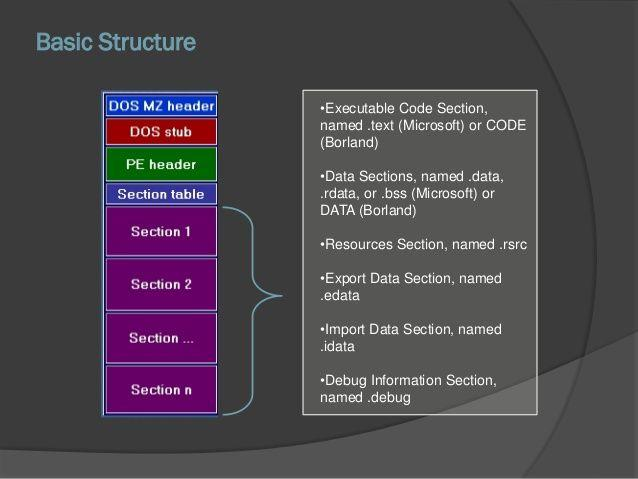
\includegraphics[width=\linewidth]{images/pe_header.jpg}
    \caption{Structure PE}
\end{figure}

    \subsubsection{En-tête MZ-DOS}
% pas sur de la phrase.
    Tout fichier PE doit commencer par l'en-tête MZ-DOS. Cet en-tête permet au système d'exploitation, au 
    moment de l'exécution d'un fichier, de reconnaître si c'est un exécutable valide ou non. \cite{pe2}

    \subsubsection{En-tête PE}
    Cet en-tête contient des champs d'information comme l'offset et la taille des zones de code et de données, 
    le système d'exploitation dont le fichier est destiné, la taille de la pile initial et 
    d'autre informations vitale. \cite{pe3}

    Les premiers bytes sont pris par MS-DOS stub qui a le rôle d'afficher un message d'erreur en cas ou 
    l'exécutable est lancé dans un environnement qui ne supporte pas Win32, les bytes suivant constitue 
    une structure de données appeler \emph{\textsc{image\_nt\_headers}} dont les champs sont :
    \begin{description}
        \item[image\_file\_header :] C'est une structure contenant les informations nécessaires
            sur le fichier comme le nombre de sections, le processeur dont le fichier est destiné \ldots etc.
        \item[image\_optional\_header :] C'est une structure contenant les des informations crucial comme l'adresse
            du point d'entrer.
    \end{description}

    \subsubsection{Les sections}
    Tous code, données et ressources sont stockés dans les sections. Une section se compose de deux 
    parties : une partie en-tête et une autre pour les données. Chaque en-tête est d'une longueur de 40 
    bytes ; il contient le nom de la section, la taille des données, l'offset de la section dans 
    le ficher PE, et l'adresse de début de la plage d'adresse du processus courant où la section doit être 
    chargé. \cite{pe4}

\section{Techniques de contournement des Anti-Virus}

% \section{Introduction}
% \section{Classification des virus par cible}
% \section{Classification des virus par techniques de dissimulations}
% \section{Les techniques d'infections}
% \section{Techniques de contournement des Anti-Virus}

\section{Conclusion}
À la fin de ce chapitre, des notions plus ou moins poussées concernant les virus --- comme les méthodes d'infections 
et les méthodes de dissimulation --- ont été abordés et étudiés. Ces notions sont indispensable pour cerner le 
mode de fonctionnement des virus, ainsi que pour la mise en œuvre du projet et du prochain chapitre.

\chapter[Développement, Injection, Propagation]{Développement du Malware et démonstration de l'injection ainsi que la propagation}
%!TEX root = ../main.tex

% Créer malware, injecter dans machine vulnérable, attendre la propagation, obtenir l'accès sur la machine sécurisé,
% une démonstration que la sécurité d'une machine dépend de la sécurité des machines avec lesquelles elle interagit.

% Tout au long de cette mémoire, nous avons parlé sur les virus, et on a cerné leurs modes de fonctionnement

Dans ce troisième chapitre, toutes les connaissances acquises durant l'étude seront mises en œuvre pour atteindre
une machine qui est supposée être sécurisée. %vérifié

La démarche que nous allons suivre est la suivante : 
\begin{itemize}
    \item Nous allons développé un Malware hybride constitué d'un virus et d'un backdoor;
    \item Le Malware sera introduit manuellement dans une machine vulnérable qui est en communication continue
        avec la machine sécurisé;
    \item Ensuit, le Malware se propagera jusqu'à la machine sécurisé sans déclencher d'alerte;
    \item Finalement, un accès total est obtenu sur la machine sécurisé par le biais du backdoor.
\end{itemize}
% nous allons développé un Malware hybride constitué d'un virus
% et d'un backdoor ; Le Malware sera introduit manuellement dans une machine vulnérable qui est en communication continue avec la machine sécurisé ; Il se propagera jusqu'à la machine sécurisé sans déclencher d'alerte ; Un 
% accès total est obtenu sur la machine sécurisé par le biais du backdoor. 

La succès de cette opération démontrera indéniablement que la sécurité d'une machine dépend toujours
de la sécurité des machines avec lesquelles elle interagit.
% machine est en communication continue avec la machine sécurisé 

% Dans cette partie de l'étude, nous allons mettre en œuvre toutes les connaissances acquises précédemment pour atteindre 
% une machine qui est supposé être sécurisé. 

% La démarche que nous allons suivre va se matérialiser dans le 
% développement d'un Malware hybride constitué d'un backdoor et d'un virus. Ce Malware sera introduit manuellement 
% dans une machine vulnérable qui est en communication continue avec la machine sécurisé. Ensuite, le Malware
% atteindra et fournira un accès sur cette dernière sans déclencher d'alerte.

% Cette démonstration a pour seul but de démontrer que la sécurité d'une machine dépend toujours de la sécurités 
% des machines avec lesquelles elle intéragit. celles avec elle
% communique

% Dans ce chapitre, nous allons mettre en œuvre toute les connaissance acquise durant cette étude pour 
% démontrer que la sécurité
% d'une machine dépend de celles avec elle communique.
\newpage

\section{Préparation de l'environnement} \label{preparation_environnement}
Dans cette section, l'environnement et les outils nécessaires pour le bon fonctionnement du projet seront installés
et préparés correctement. Il y en a en gros trois machines différentes : une machine d'attaque, une machine vulnérable,
et finalement une machine sécurisée. %vérifié

    \subsubsection{La machine d'attaque} 
    Cette machine sera équipée du système d'exploitation \emph{Kali Linux \cite{linux} Rolling} 
    (\autoref{kali_linux}), le 
    leader des systèmes de test d'intrusions. Après le téléchargement de l'image
    ISO depuis le site officiel de Kali, et l'installation de l'image sur
    une machine virtuelle, une mise à jour complète du système est faite par le biais de cette commande : 
    ``\texttt{sudo apt-get update \&\& sudo apt-get upgrade}''  %vérifié

    \begin{figure}[h!]
        \centering
        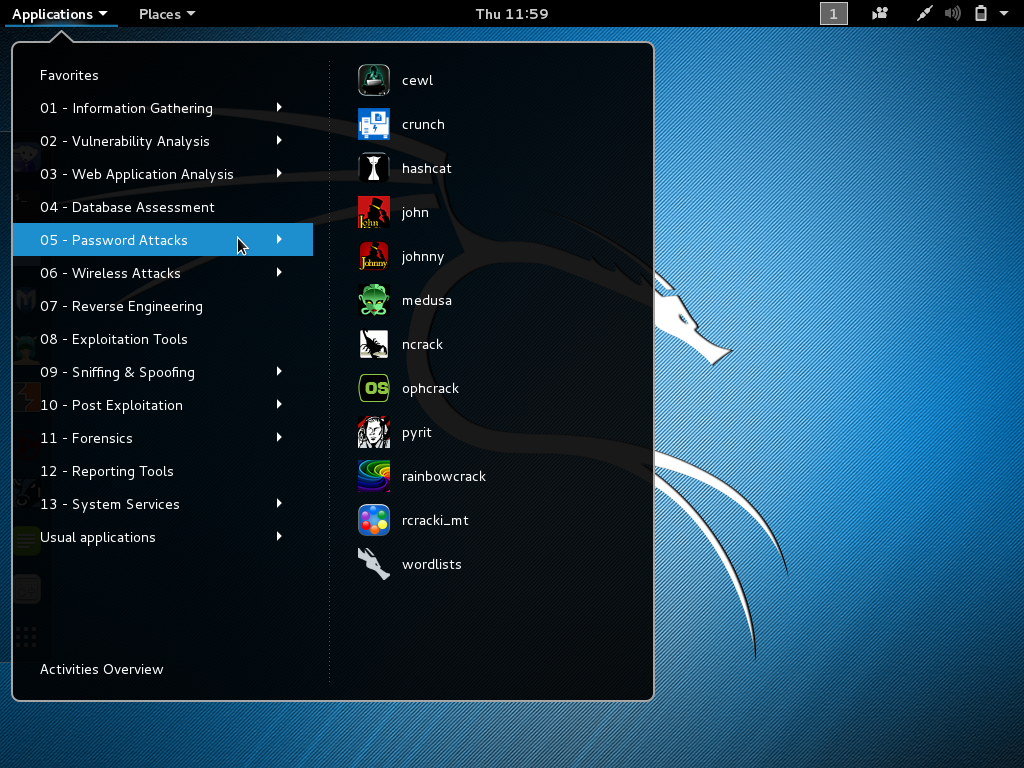
\includegraphics[width=\linewidth]{images/kali_linux.png}
        \caption{Kali Linux}
        \label{kali_linux}
    \end{figure}

    \subsubsection{La machine vulnérable} \label{machine_vulnerable} 
    Cette machine sera équipée d'une version \emph{Windows 7}  
    dotée d'un service vulnérable et d'un pare-feu désactiver. Le service vulnérable installé sur cette 
    machine est un service \emph{FTP} manipulé par le programme \emph{KONICA MINOLTA FTP Utility} 
    (\autoref{la_machine_vulnerable}). %vérifié
    \begin{figure}[h!]
        \centering
        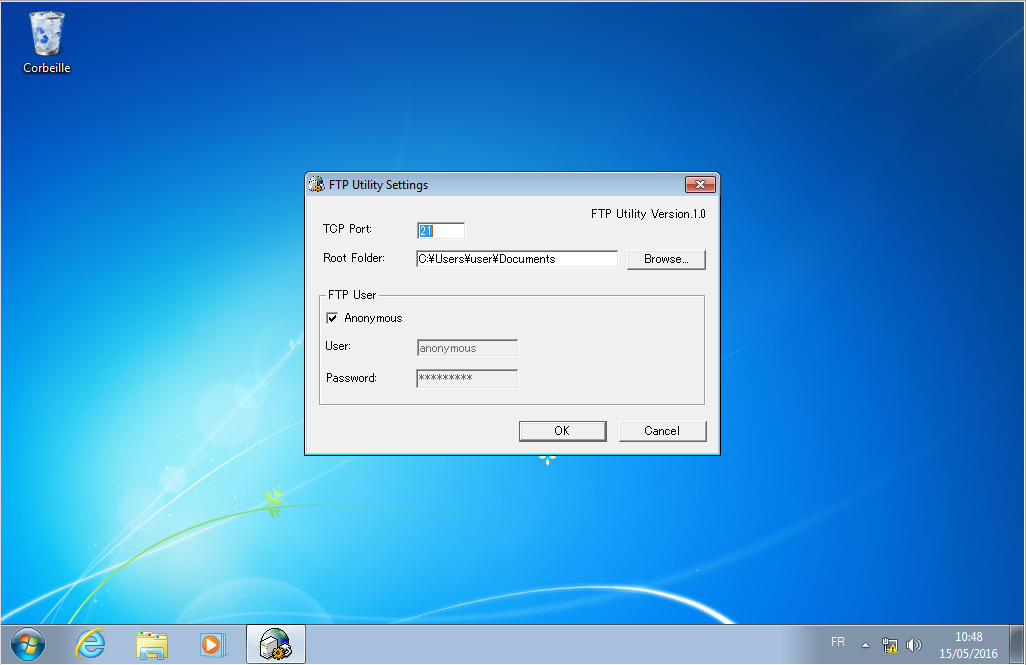
\includegraphics[scale=0.3]{images/Windows_7_2.png}
        \caption{La machine vulnérable}
        \label{la_machine_vulnerable}
    \end{figure}

    \subsubsection{La machine sécurisée} 
    Cette machine sera équipée de \emph{Windows 7} avec la dernière version de l'anti-virus \emph{Kaspersky} 
    dont la base de données a été mise à jour (\autoref{mise_a_jour_kaspersky}). %vérifié

    \begin{figure}[!h]
        \centering
        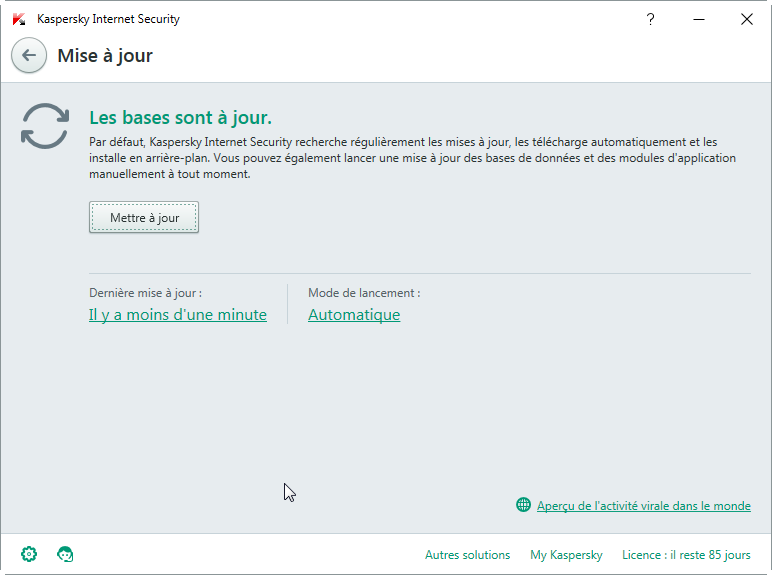
\includegraphics[width=\linewidth]{images/mise_a_jour_kaspersky.png}
        \caption{Mise à jours Kaspersky}
        \label{mise_a_jour_kaspersky}
    \end{figure}

\subsection{Réseau}
    Les trois machines seront dans le réseau \cite{reseau} dont l'adresse est \emph{172.16.178.0/24}. 
    La machine d'attaque aura l'adresse IP \emph{172.16.178.1} ; la machine vulnérable aura l'adresse IP 
    \emph{172.16.178.129} ; et finalement, la machine sécurisée aura l'adresse IP \emph{172.16.172.130}. %vérifié

    Pour voir comment le réseau a été configuré sur chaque machine, consultez \autoref{config_reseau}. %vérifié


\section{Développement}
    \subsection{Backdoor}
    Dans cette section, deux programmes seront développés : un programme qui s'exécutera sur la machine victime
    qui représentera le backdoor , et un autre qui s'exécutera sur la machine assaillante. %vérifié
    % Malgré qu'en général, exécuter un backdoor sur la machine victime et utiliser un logiciel de communication réseau
    % (comme netcat \autoref{netcat}),
    % est amplement suffisant pour obtenir un accès ; mais pour plus de compatibilité, nous allons développer 
    % les deux parties, qui sont : le backdoor et le programme qui permettra de communiquer avec.
    % le backdoor et le programme qui permettra de communiquer avec. nous allons nous même 
    % créer un programme qui permettra de communiquer avec le backdoor. 

    % Malgré que le strict minimum de cette section exige qu'on développe un backdoor (porte dérobé \autoref{backdoor})
    % qui fournira un accès à la machine victime, mais nous allons quand même développer un petit programme du côté 
    % de l'attaquant, un programme qui permettra de communiquer avec le backdoor.

    % Donc, deux programmes seront développés dans cette section : Un programme pour la machine assaillante, et 
    % un backdoor qui s'exécutera sur la machine victime.
        \subsubsection{Côté victime}
        Pour plus de discrétion, on va utiliser une technique appelée \emph{reverse connection} pour établir la connexion
        avec le backdoor. %vérifié
        % Pour éviter tous problèmes avec le pare-feu, on va utiliser une technique appelé \emph{reverse tcp}. 

        En d'autres termes, au-lieu que le backdoor ouvre un port et attend qu'on se connecte à ce port pour 
        communiquer avec lui, il va plutôt essayer d'établir une connexion vers nous. Cela permettra d'éviter la demande
        d'ouverture d'un port au pare-feu et l'éveille des soupçons de l'administrateur de la machine ; 
        par conséquence, le backdoor sera encore plus difficile à détecter.
        % Ça passe plus inaperçu, et 
        % ça évite la demande d'ouverture d'un port au pare-feu (ce qui est une activité suspecte).

        En ce qui concerne le fonctionnement du backdoor, celui-ci a été simplifié le plus possible, pour que 
        l'infection (\autoref{virus_infecteur}) passe inaperçu, et lui donner plus de chance d'échapper aux yeux des anti-virus. 
        Malgré que les fonctionnalités ont été limitées, on a donnée quand même la chance à notre backdoor 
        d'évoluer et d’intégrer plus de fonctionnalité par la suite, comment on a fait cela ? 
        L'explication est abordée ici avec la liste des fonctionnalités proposées par le backdoor : %vérifié

        \begin{description}
            \item[Accès sécurisé :] Dés le moment où le backdoor établi la connexion, un mot de passe est
                demandé par ce dernier (\autoref{backdoor_password}); si le mot de passe renseigné est correct, 
                alors l'accès est accordé, sinon la connexion est arrêter immédiatement. %vérifié

                \begin{figure}[h!]
                    \centering
                    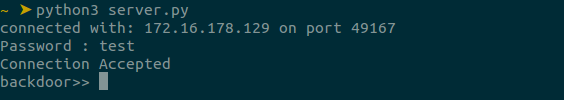
\includegraphics[width=0.9\linewidth]{images/backdoor_password.png}
                    \caption{Demande de mot de passe}
                    \label{backdoor_password}
                \end{figure}

                Pour éviter que le mot de passe soit découvert en \emph{désassemblant} l'exécutable du backdoor,
                une version hachée est conservé et utilisé pour valider le mot de passe fournie au moment de la 
                connexion. %vérifié

            \item[Accès à l'invite de commande :] Avec cette fonctionnalité, 
                chaque message envoyé par nous est redirigé vers la ligne 
                de commande de Windows, et la réponse de cette dernière est alors renvoyée.
                \begin{figure}[h!]
                    \centering
                    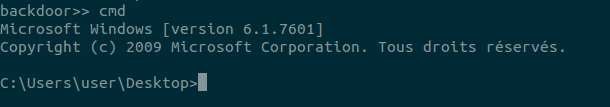
\includegraphics[width=0.9\linewidth]{images/backdoor_cmd.png}
                    \caption{Invite de commande}
                    \label{backdoor_cmd}
                \end{figure}

            \item[Envoi et réception de fichiers :] Cette fonctionnalité nous permet d'échangé des fichiers 
                avec le backdoor. Ainsi, on pourra envoyer et recevoir des fichiers depuis la machine victime.

            \item[Mettre à jours le backdoor :] Cette fonctionnalité nous permet d'étendre les fonctionnalités du
                backdoor, en le remplaçant par un autre plus sophistiqué et plus complet. Il a été précisé 
                précédemment qu'on a fait exprès de créer un backdoor simple pour éviter qu'il soit détecté ; mais 
                avec cette fonctionnalité, la seule limite de notre backdoor est notre imagination.
        \end{description}

        En ce qui concerne le lancement du backdoor, ce dernier sera lancé périodiquement par le virus, pour 
        diminuer les chances qu'une inspection des communications réseau puisse découvrir sa présence.
        % Cela permettra 
        % d'éviter la consommation inutile des ressourcesla consommation des ressources
        % Pour encore plus de discrétion, le backdoor ne sera pas en marche sans arrêt, mais il sera plutôt lancé chaque
        % période de temps par le virus.

        \subsubsection{Côté assaillant}
        Malgré qu'en général, utiliser un logiciel de communication réseau (comme netcat \autoref{netcat}) 
        est amplement suffisant pour communiquer avec 
        le backdoor. Sauf que pour exploiter toutes les fonctionnalités de ce dernier, il est indispensable 
        de développé un programme qui permettra de communiquer avec. 

        Ce programme, ou plutôt ce script python \cite{python}, écoutera sur un port donnée, et attendra la connexion du backdoor.
        Une fois cette dernière est établie, ce script permettra d'envoyer des commandes, et de recevoir leurs réponses.
        % Ce programme, ou plutôt ce script python, est extrêmement simple ; son unique tâche et d'écouter sur un port 
        % donnée, et attendre la connexion du backdoor. Une fois la connexion établie, il permettra d'envoyer 
        % des commandes, et de recevoir leurs réponses.

        \subsubsection{Backdoor amélioré}

        Ce backdoor, en plus d'intégrer toutes les fonctionnalités de l'ancien backdoor, il établie une connexion 
        crypté basé sur le protocole \emph{TLS}\footnote{Le \emph{TLS} (\emph{Transport Layer Security})
        est un protocole de sécurisation des communication réseau.}.

        Pour démonstration, le logiciel \emph{Wireshark}\footnote{\emph{Wireshark} est un analyseur de 
        paquets réseau multi-plateforme supportant plusieurs centaines de protocoles. Il permet d’examiner les 
        données qui transitent sur le réseau, et par conséquence voir le contenu des paquets en direct et en détails.} 
        a été utilisé pour montrer la différence entre la communication 
        en claire utilisé par le premier backdoor (\autoref{communication_claire})
        , et la communication cryptée utilisé par le backdoor amélioré (\autoref{communication_cryptee}).

        \begin{figure}[!h]
            \centering
            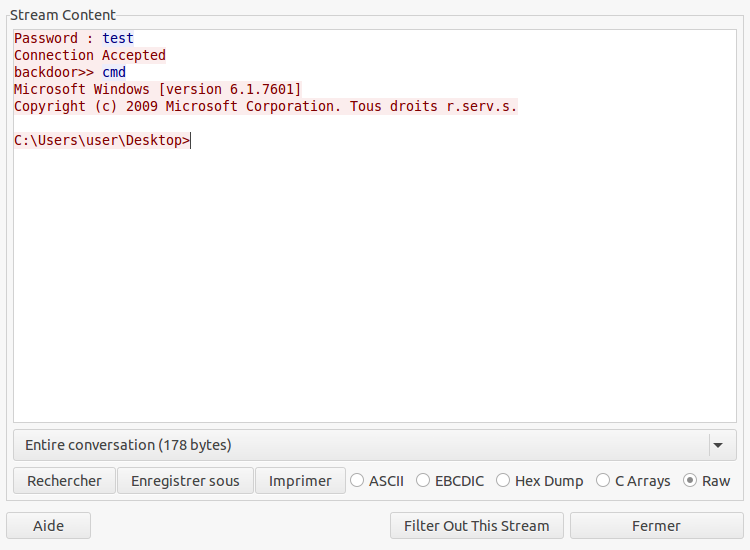
\includegraphics[width=0.8\linewidth, height=250pt]{images/communication_claire.png}
            \caption{Communication en claire}
            \label{communication_claire}
        \end{figure}
        \begin{figure}[!h]
            \centering
            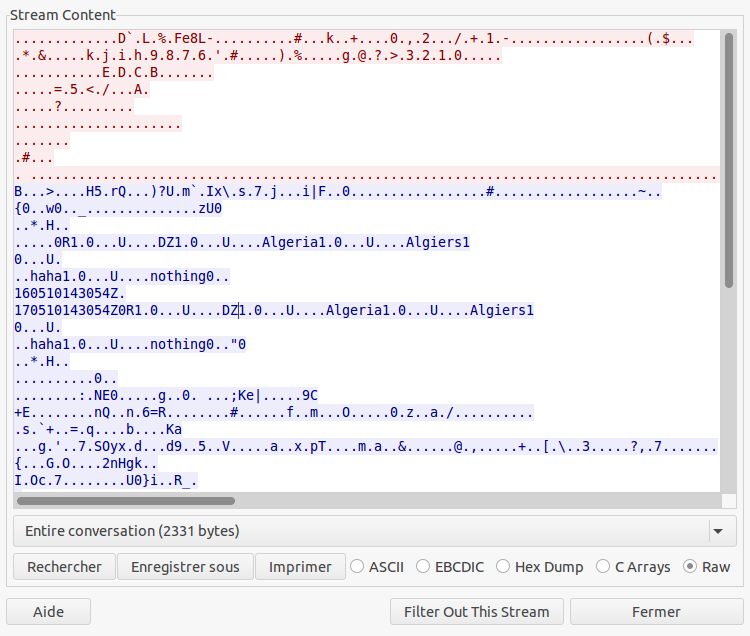
\includegraphics[width=0.8\linewidth, height=250pt]{images/communication_cryptee.png}
            \caption{Communication crypté avec le protocole TLS}
            \label{communication_cryptee}
        \end{figure}

        % non seulement il contient toutes les fonctionnalités de l'ancien backdoor, mais en
        % Ceci une petite démonstration sur la possibilité que nous offres la fonctionnalité de mise à jour. Dans cette
        % démonstration, l'ancien backdoor sera remplacé par le backdoor amélioré.
        % Le backdoor amélioré prendra la place de l'ancien backdoor dans le processus de mise à jour. 

        % En plus des fonctionnalités de l'ancien backdoor, le backdoor amélioré établira une connexion sécurisé 
        % basé sur le protocole SSL ; ainsi, l'échange sera crypté, et une inspection des paquets qui circulent sur
        % le réseau ne donnera rien de spécial.

    \subsection{Virus} \label{virus_infecteur}
    La méthode d’infection que nous allons utiliser est : l’injection de code dans un exécutable par \emph{Ajout}
    dont une définition claire a été abordée dans la \autoref{infeciton_ajout}.

    Cette technique, se base sur la manipulation de la structure PE (une définition détaillée a été donnée dans le 
    \autoref{pe_header}), nous avons donc inclus la bibliothèque \emph{Windows.h} qui contient les 
    structures et fonctions nécessaires.

    Le code se divise en deux fonctions primordiales :
    \begin{description}
        \item[WinMain :] Cette fonction est la fonction Main, dans un premier temps son rôle est de créer 
        deux espaces mémoire pour y stocker le code du Virus et du Backdoor, puis de cibler un exécutable. 
        une vérification sera faite sur sa compatibilité avec Windows 32 bits.

        Dans un deuxième temps, elle ouvre ce dernier et récupère sa structure PE. Après des calculs précis, 
        elle stocke dans une variable le Point d’Entrer Original appelé \emph{OEP} et ajoute à la fin de ce 
        fichier deux nouveaux segments; le segment qui contient le code du Virus et un autre qui contient 
        le code du Backdoor puis les crypte avec une clé prédéfinie. A la fin, elle 
        change le point d’entrer et le fait pointer vers la fonction VirusCode (\autoref{entrypoint_changement}).
        La fonction modifie aussi le \emph{loader flags}\footnote{\emph{loader flags} est un flag obsolète non
        utiliser par Windows comme expliqué dans ce lien \url{https://msdn.microsoft.com/en-us/library/windows/desktop/ms680339(v=vs.85).aspx}.} et y place notre flag d'infection. En dernier, une correction du \emph{Checksum}
        sera faite.
        
        \item[VirusCode :] Cette fonction sera le nouveau point d’enter de chaque exécutable infecté, 
            elle s’exécutera toujours en premier puis elle donnera la main au code original, 
            elle passe par trois étapes clé :

            Premièrement, puisque cette fonction n'a pas été compiler avec l’exécutable hôte, elle ne connais pas les adresse des fonctions qu'elle va utilise,
            donc une récupération de l’adresse de la bibliothèque Kernel32
            chargé avec l’exécutable hôte est primordiale et suffisant pour trouver et stocker les
            adresses des fonctions nécessaires au bon fonctionnement du code malveillant.

            Deuxièmement, elle chargera l’adresse du segment du Virus et du Backdoor, créera deux 
            emplacements mémoire et les copie dedans, puis elle les décrypte.

            Et enfin, elle créera deux fichiers exécutables dans le dossier “temp”, un contenant le Virus et 
            l’autre le Backdoor, et les exécutera. En dernier, un appel vers le point d’entrer original sera fait
            pour redonner la main à l'exécutable hôte, ce qui permettra d'éviter l'éveille des soupçons.

    \end{description}

\newpage

    \begin{figure}[H]
        \centering
        \begin{subfigure}{0.9\textwidth}
            \centering
            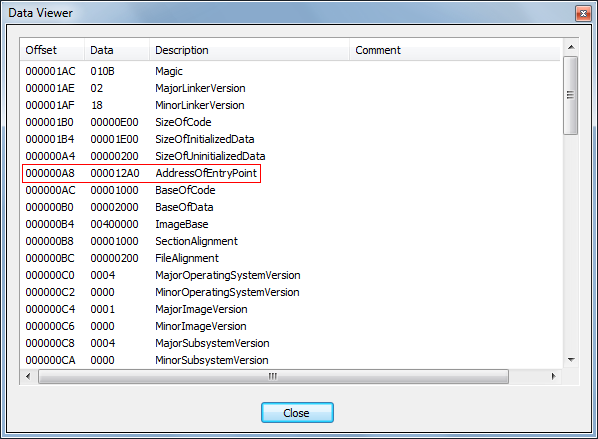
\includegraphics[width=\textwidth]{images/entrypoint_avant.png}
            \caption{Point d'entrée avant infection}
            \label{entrypoint_avant}
        \end{subfigure}
        \hfill
        \begin{subfigure}{0.9\textwidth}
            \centering
            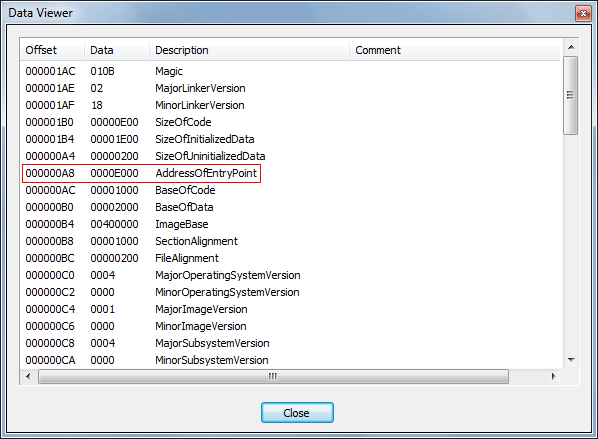
\includegraphics[width=\textwidth]{images/entrypoint_after.png}
            \caption{Point d'entrée après infection}
            \label{entrypoint_apres}
        \end{subfigure}
        \hfill
        \caption{Changement du point d'entrée de l'exécutable}
        \label{entrypoint_changement}
    \end{figure}

    Nous citerons aussi que ce Virus infecte les fichiers exécutables des clés USB connecté à la machine.
    La particularité majeure de notre Virus est qu’il utilise des API native, et qu’il ne peut pas être 
    déboguer, une démonstration est montrer dans la figure suivante:

\section{Exploitation} \label{exploitation}
Cette section sera consacré à l'exploitation de la machine vulnérable, et l'obtention d'un accès à distance
sur cette dernière. On commencera par une bref présentation des outils utilisés pour une meilleur compréhension
de cette section.
    \subsection{Présentation des outils}
    \begin{description}
        \item[netcat :] \label{netcat}
            C'est un outil utilisé en ligne de commande, et qui permet l'ouverture des connexions
            réseau, que ce soit \emph{TCP} \cite{reseau} ou \emph{UDP} \cite{reseau}. En raison de sa polyvalence,
            il est aussi appelé le \emph{couteau suisse} du réseau.

            Pour se connecter à un serveur sur un port donnée, il faut donner à \emph{netcat} deux paramètres qui sont 
            l'adresse du serveur et le port qu'utilise le serveur. Exemple :
            \begin{lstlisting}[language=bash] 
            $ netcat www.google.com 80
            \end{lstlisting}

            Dans le côté serveur, pour mettre netcat en écoute sur un port, il faut préciser deux options qui sont 
            `\emph{-l}' pour dire à netcat d'écouter, et `\emph{-p \ul{port}}' pour préciser le port d'écoute.
            Exemple :
            \begin{lstlisting}
            # netcat -l -p 80   
            \end{lstlisting}

        \item[Metasploit :] C'est un \emph{Framework} de testes de pénétrations \emph{open source} utilisé pour 
            tester la robustesse des machines en matière de sécurité. Il est composé essentiellement de charges 
            et d'exploits. 

        \item[msfvenom :] \label{msfvenom} C'est un générateur et encodeurs de charges. Il est utile pour une utilisation plus manuelle
            des charges, car il permet de générer ces dernières dans plusieurs format (des exécutables, pour un 
            script python \ldots{}). 

            Plusieurs paramètres sont à utiliser pour obtenir des charges plus performantes. Parmi ces options on y
            trouve :
            \begin{description}
                \item[-a \ul{architecture} :] L'architecture du système dont la charge est destiné
                    (x86 ou x64).
                \item[--plateform \ul{plateforme} :] Le système attaqué (Windows, Mac, Linux, Android
                \ldots{}).
                \item[-p \ul{charge} \ul{options\_de\_la\_charge}:] La charge et les options utilisés 
                    pour générer celle-ci.
                \item[-e \ul{encodage} :] L'encodage utilisé pour générer la charge.
                \item[-b \ul{mauvais\_octets} :] Les octets à éviter pendant la génération de la charge.
                \item[-f \ul{format} :] Format de la charge (exécutable, python, perl \ldots{}).
            \end{description}

        \item[meterpreter :] \label{meterpreter}C'est une charge avancée et extensible développé par les développeurs de 
            \emph{Metasploit}. Elle est utilisé par ce dernier pour donner un accès plus étendu et plus 
            complet à une machine exploitable. 
    \end{description}

    \subsection{La vulnérabilité}
    Le programme vulnérable qu'on va exploiter se nomme \emph{Konica Minolta FTP Utility} (\autoref{konica_minolta}). 
    C'est un programme qui utilise le protocole \emph{FTP}\footnote{Le \emph{FTP} est un protocole destiné
    à l'échange informatique des fichiers sur un réseau.} pour la réception des données depuis des appareils 
    compatibles. La version vulnérable, qui est la \emph{version1.0} 
    (la dernière jusqu'à maintenant), peut être obtenu depuis ce lien 
    \url{https://www.exploit-db.com/apps/6388a2ae7dd2965225b3c8fad62f2b3b-ftpu_10.zip}.
    % La version vulnérable du programme est la \emph{version 1.0} (qui est la dernière version 
    % jusqu'à maintenant), cette version peut être obtenu depuis ce lien 
    % \url{https://www.exploit-db.com/apps/6388a2ae7dd2965225b3c8fad62f2b3b-ftpu_10.zip}.
    % pour recevoir des données 
    % Le service vulnérable qui a été installé est un service \emph{ftp} manipulé par le programme 
    % \emph{Konica Minolta FTP Utility}. 

    \begin{figure}[h]
        \centering
        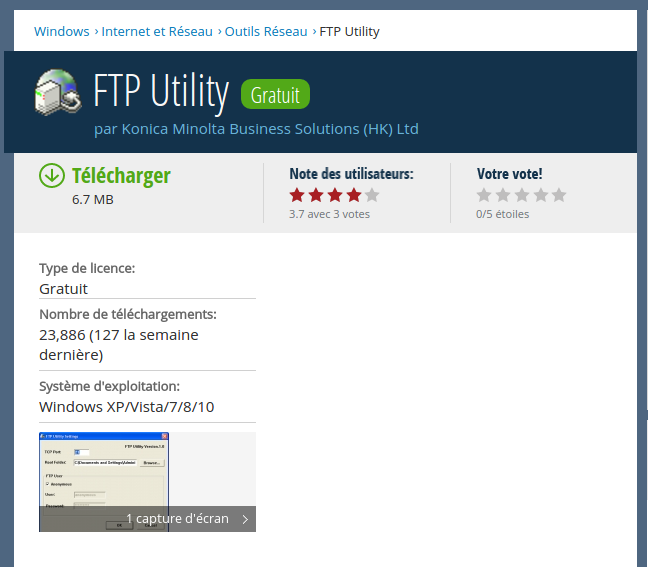
\includegraphics[width=0.8\linewidth]{images/konica_minolta.png}
        \caption{Konica Minolta FTP Utility}
        \label{konica_minolta}
    \end{figure}

    La vulnérabilité découverte dans ce programme est un débordement de tampon (\autoref{buffer_overflow}), 
    elle a été publié le 21 Janvier 2016 sur le site d'\emph{Exploit Database} 
    \footnote{\emph{Exploit Database} est un site qui se charge d'archiver les exploits publics et les 
    logiciels vulnérables correspondants. Ce site dont le lien est \url{www.exploit-db.com} est développé 
    par les testeurs d'intrusions et les chercheurs de vulnérabilités.} par un contributeur surnommé \emph{TOMIWA}.
    % La vulnérabilité découverte, qui est un débordement de tampon (\autoref{buffer_overflow}), a été publié le 11
    % Janvier 2016 sur le site d'\emph{Exploit Database}\footnote{\emph{Exploit Database} est un site qui se charge
    % d'archiver les exploits publics et les logiciels vulnérables correspondants. Ce site dont le lien est 
    % \url{www.exploit-db.com} est développé par les testeurs d'intrusions et les chercheurs de vulnérabilités.} 
    % par une personne surnommé \emph{TOMIWA}.

    % La vulnérabilité est présente dans la \emph{version 1.0} (qui est la dernière version jusqu'à maintenant) du
    % programme. Cette version peut être obtenu depuis ce lien 
    % \url{https://www.exploit-db.com/apps/6388a2ae7dd2965225b3c8fad62f2b3b-ftpu_10.zip}.

    \subsection{L'exploit}
    Le script qui permet d'exploiter cette vulnérabilité peut être récupérer depuis ce lien 
    \url{https://www.exploit-db.com/exploits/39215/}.
    Ce script \emph{python} \cite{python} se divise en deux parties :
    \begin{description}
        \item[Exploit :] Cette partie du script permet en quelque sorte de préparer le programme vulnérable à 
            recevoir le code malveillant pour l'exécution. Cette partie n'est pas à modifier, car elle a été développé
            après une étude approfondie du programme vulnérable.

        \item[Charge :] Cette partie du script représente le code qui sera exécuté sur l'application vulnérable. 
            Cette partie peut être remplacé par la charge désiré par l'attaquant.
            % L'exploit téléchargé depuis ce lien \url{https://www.exploit-db.com/exploits/39215/} vient avec une charge
            % par défaut, qui est un \emph{reverse shell}.% Pour notre démonstration, on ne va pas utiliser 
            % la charge par défaut, mais on va plutôt utiliser une autre charge qui permet d'exécuter un programme 
            % beaucoup plus puissant, qui est \emph{meterpreter}. 
    \end{description}

    Le script va se connecter à la machine victime sur le port 21 (\autoref{execution_script_exploitation}). 
    La charge qu'utilise le 
    script va ordonné à la machine qu'elle donne un reverse shell en se reconnectant à la machine de l'attaquant 
    sur le port 4444. Pour intercepter ce reverse shell, et pouvoir communiquer avec
    la machine victime, il faut ordonner à netcat d'écouter sur le port 4444 (\autoref{obtention_reverse_shell}).

    \begin{figure}[h!]
        \centering
        \begin{subfigure}{0.9\textwidth}
            \centering
            
\includegraphics[width=\textwidth]{images/exploit_python.png}
            \caption{Exécution du script d'exploitation}
            \label{execution_script_exploitation}
        \end{subfigure}
        \hfill
        \begin{subfigure}{0.9\textwidth}
            \centering
            
\includegraphics[width=\textwidth]{images/reverse_shell.png}
            \caption{Obtention du reverse shell}
            \label{obtention_reverse_shell}
        \end{subfigure}
        \hfill
        \caption{Exploitation avec la charge d'origine}
        \label{exploitation_avec_charge_origine}
    \end{figure}

    La charge par défaut de ce script est une charge un petit peu limitée, donc nous allons nous en servir 
    de \emph{msfvenom} pour générer la charge \emph{meterpreter} (\autoref{generation_charge}) et l'utiliser 
    dans le script d'exploitation.
    \begin{figure}[h]
        \centering
        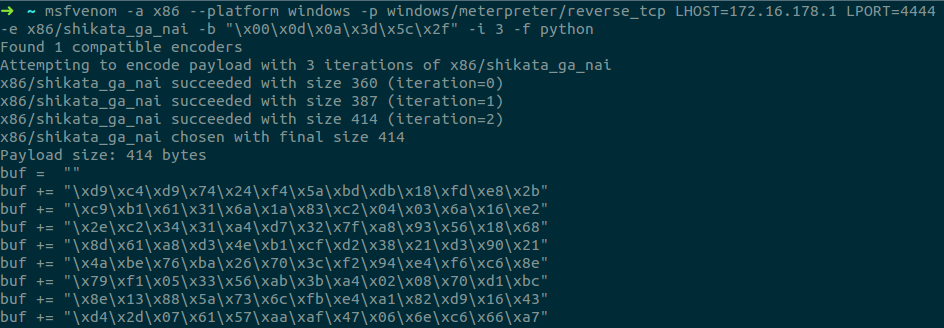
\includegraphics[width=\linewidth]{images/msfvenom.png}
        \caption{Génération de la charge}
        \label{generation_charge}
    \end{figure}

    \subsection{Obtention d'accès}
    Pour la charge utilisé précédemment, il a suffit d'utiliser netcat pour intercepter la connexion et communiquer
    avec la machine victime. Mais meterpreter exige des techniques plus poussées pour pouvoir faire cela, 
    donc nous allons faire appel aux services de Metasploit pour accomplir cette tâche.
    On commence par lancer Metasploit en mode console (\autoref{msfconsole}) par le biais de la commande 
    `\emph{msfconsole}'. Après, on effectue les manipulations nécessaires (\autoref{config_metasploit})
    pour pouvoir intercepter les réponses de meterpreter.

    \begin{figure}[H]
        \centering
        \begin{subfigure}{0.9\textwidth}
            \centering
            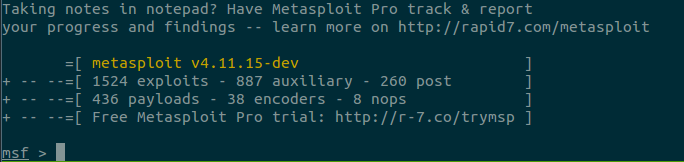
\includegraphics[width=\textwidth]{images/msfconsole.png}
            \caption{Lancement de Metasploit}
            \label{msfconsole}
        \end{subfigure}
        \hfill
        \begin{subfigure}{0.9\textwidth}
            \centering
            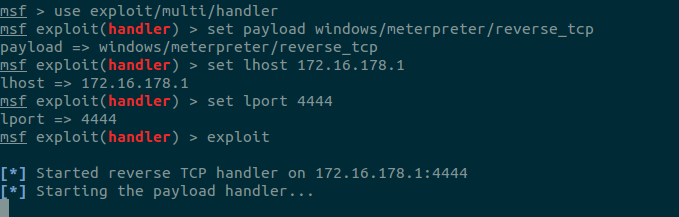
\includegraphics[width=\textwidth]{images/ecoute_msf.png}
            \caption{Configuration de Metasploit}
            \label{config_metasploit}
        \end{subfigure}
        \hfill
        \caption{Préparation de Metasploit}
        \label{prepration_metasploit}
    \end{figure}

    Maintenant, il ne reste plus qu'à lancer le script d'exploitation qu'on a modifié et obtenir un accès à la 
    machine exploité (\autoref{obtention_accees_meterpreter}).

    \begin{figure}[H]
        \centering
        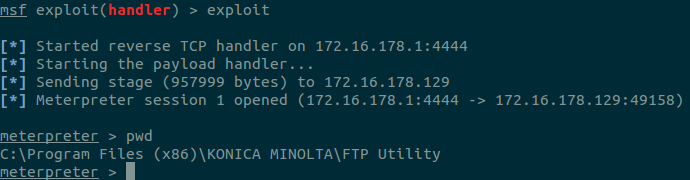
\includegraphics[width=\linewidth]{images/meterpreter.png}
        \caption{Obtention de l'accès avec meterpreter}
        \label{obtention_accees_meterpreter}
    \end{figure}

\section{Teste de propagation}
Cette partie contiendra une simulation de propagation du Malware développée au cours de ce projet, et 
l'infection des machines d'une entreprise virtuel,

Pour cela, nous procédons au test sur l’environnement cité auparavant dans la \autoref{preparation_environnement}.

Tout d'abord, nous exploitons la vulnérabilité présente dans la machine de faible sécurité, pour avoir accès au Shell de cette dernière (comme expliqué dans la \autoref{exploitation}), de ce fait, nous envoyons notre Malware puis nous l’exécutons (\autoref{launch_virus})

\begin{figure}[H]
    \centering
    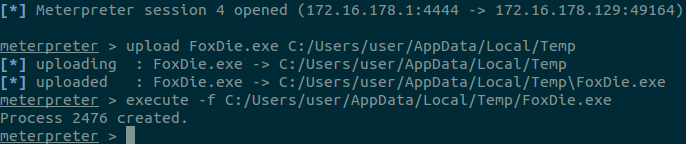
\includegraphics[width=\linewidth]{images/exec_virus.png}
    \caption{Envoi et exécution du virus}
    \label{launch_virus}
\end{figure}
Cela infectera la machine et tout fichier exécutable contenu dans des périphériques de stockage externe qui sont, ou qui vont  être connectes à cette machine.  Nous pouvons constater que le processus de notre Virus est en execution sur la machine, et nous pouvons aussi observer qu'à chaque minute, le backdoor est exécuté (\autoref{process_backdoor}).

\begin{figure}[H]
    \centering
    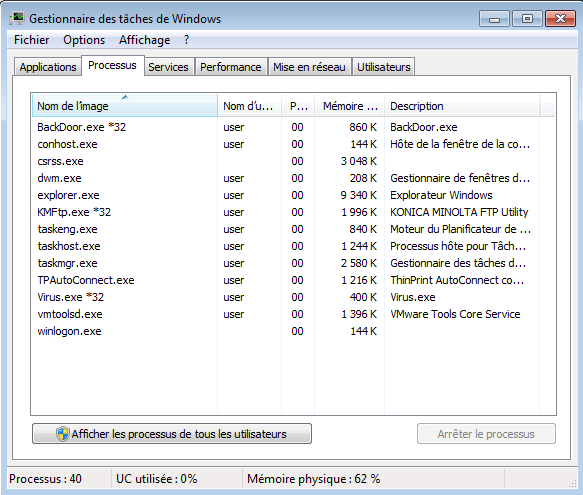
\includegraphics[width=\linewidth]{images/processus_backdoor.png}
    \caption{Processus du backdoor}
    \label{process_backdoor}
\end{figure}

Pour la deuxieme étape de notre test, nous connectons une clé usb contenant plusieurs fichiers, dont des exectuables et autres (\autoref{avant_infection}). A ce titre nous pouvons constater que la taille des executables s'agrandit de 144 Ko (\autoref{apres_infection}), cela veux dire que les deux segments (le virus et le backdoor) ont été ajouté correctement .

\begin{figure}[H]
    \centering
    
\includegraphics[width=\linewidth]{images/avant_infeciton.png}
    \caption{Avant Infection}
    \label{avant_infection}
\end{figure}

\begin{figure}[H]
    \centering
    
\includegraphics[width=\linewidth]{images/apres_infection.png}
    \caption{Après Infection}
    \label{apres_infection}
\end{figure}

Nous prenons cette clé, puis nous la connectons à la machine qui est hautement sécurisée. Nous essayons de l'analyser avec le fameux Anti Virus \emph{Kaspersky} qui après analyse indique que tous les fichiers contenus dans la clé sont sains et non infectés (\autoref{scan_cle}). Nous procédons alors à l’exécution de l'un des fichiers exécutable comme le ferait n'importe quel usager utilisant un Anti Virus.

\begin{figure}[H]
    \centering
    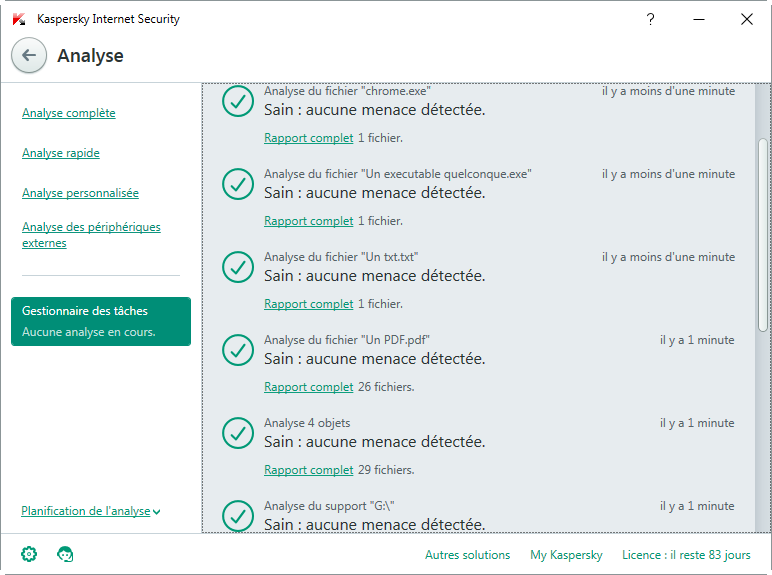
\includegraphics[width=\linewidth]{images/scan_by_antivirus.png}
    \caption{Scan de la clé USB}
    \label{scan_cle}
\end{figure}

A cet effet, le code malveillant contenu dans le logiciel infecté s’exécute en premier comme cité dans la 
\autoref{virus_infecteur}, et fera la tâche qui lui a été assignée.

Par la suite, nous lançons  notre serveur dans notre machine en écoute comme le montre la figure suivante, et on attend que le backdoor qui s’exécute dans la machine sécurisée se connecte vers ce dernier. Après un laps de temps, la connexion s'effectue (\autoref{connect_backdoor}), ce qui nous donne finalement un accès total à la machine réputée comme étant protégée et inviolable.

\begin{figure}[H]
    \centering
    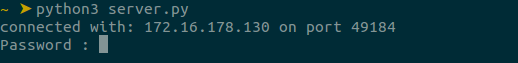
\includegraphics[width=\linewidth]{images/backdoor_connect.png}
    \caption{Connexion du backdoor à notre serveur}
    \label{connect_backdoor}
\end{figure}

\section{Conclusion}
A la fin de chapitre final, nous avons réuissi à dévellopé un Malware hybride. Ce Malware a prouvé son efficacité
contre les anti-virus, et il a réussi à atteindre la machine sécurisé par le biais d'une propagation furtive.

A la fin de chapitre, une machine sécurisé à été atteinte par notre Malware. Pour 
parvenir à cet objectif, nous avons commencé par développé le Malware hybride, puis, il a été 
injecté dans la machine vulnérable par le biais de l'exploitation d'une faiblesse dans cette dernière. 
Enfin, le Malware a réuissi à propager jusqu'à la machine sécurisé en car elle est en communication 
continue avec la machine qu'on a exploité précédemment.

% A la fin de chapitre final, nous avons réussi à atteindre une machine sécurisé par le moyen d'un Malware que nous 
% avons développé. Ce Malware s'est propagé jusqu'à atteindre 

% A la fin de ce chapitre final nous avons développé le Malware avec succès, tester son efficacité contre les Anti-Virus, et tester sa propagation vers des machines plus sécurisé.
% Il reste qu’il est toujours possible d’optimiser l’efficience du Malware au vue de sa capacité a évité les Anti-Virus.


\chapter*{Conclusion Générale}
\addcontentsline{toc}{chapter}{\protect\numberline{}Conclusion générale}
%!TEX root = ../main.tex

Ce projet de fin d'études a été riche en enseignements, qui nous a introduit dans le monde de la sécurité informatique 
et nous a permis en tant qu'étudiants d'apprendre les principes de base de la discipline tout cela en développant un 
Malware hybride.

Tout d'abord, nous avons introduit quelques notions de base sur la sécurité et les Malwares, puis nous nous sommes 
étalés sur les techniques d'infection virale.

En second lieu, notre travail a consisté à concevoir et à mettre en œuvre un Malware hybride, dont la tâche est 
d'infecter les exécutables contenus dans les périphériques de stockage externe d'une machine en s'injectant dedans et 
de fournir une porte dérobée pour un futur accès distant à la machine. Son développement a nécessité l'apprentissage 
des langages de programmation dont le C, le Python et bien sûr, l'assembleur. Nous avons aussi appris a manipulé les 
logiciels de désassemblage tels que : IDA et Ollydbg.

Finalement, nous avons simulé un environnement d'une entreprise, où une machine qui présente une vulnérabilité a été 
exploitée et infecter par notre Malware, donnât que cette machine communique en interne avec les maillons fort, 
cela a mené à la propagation de ce dernier, et l'infection des machines de l'entreprise.

De ce fait, nous avons démontré que la sécurité de chaque machine dépend de celle avec qui elle communique.

Dans notre processus de travail, nous avons appris le travail de groupe et la répartition des tâches, aussi des
connaissances de qualité qui étaient nouvelles pour nous ont été acquise. À partir de là, nous avons pu contempler 
le monde de la sécurité informatique, ce qui nous a poussé à vouloir poursuivre notre parcours universitaire et 
professionnel dans le domaine de la \emph{Sécurité des Systèmes d'Informations}.

\appendix
%!TEX root = ../main.tex

\chapter{Configuration du réseau} \label{config_reseau}

% \chapter{Los commandes utilisées} \label{commandes}

% \chapter{Codes sources} \label{code}

% \chapter{Installation d'Ubuntu} \label{install_ubuntu}

\bibliographystyle{unsrt} %ieetr
\bibliography{references}
% \printbibliography

\end{document}